\chapter{Desarrollo de la solución}\label{CAP6}
    
    
    En este capitulo se explica la solución adoptada para validar la cinemática y dinámica de un robot delta. Para ello implementan 3 herramientas a este trabajo: ROS, RVIZ y ADAMS. 
    
    \begin{figure}[h]
        \centering
        \smartdiagram[bubble diagram]{Solucion,ROS,RVIZ,ADAMS}
        \caption{Caption}
        \label{fig:cap6_intro_1}
    \end{figure}

    Se sigue una serie de pasos para validad la cinemática y dinamica del robot delta:
    
    \begin{enumerate}
        \item ROS y RVIZ
            \begin{itemize}
                \item {Trayectoria: Se crear trayectoria lineal (trapezoidal) en el espacio cartesiano $XYZ$ , velocidad $\dot{X}\dot{Y}\dot{Z}$ y aceleración $\ddot{X}\ddot{Y}\ddot{Z}$ del centroide del efector a partir de un punto inicial $P_i(x,y,z)$, un punto final $P_f(x,y,z)$, velocidad maxima $v_{max}$ y aceleración maxima $a_{max}$ deseada}
                \item {Cinemática inversa: Se calcular la trayectoria en el espacio articular $\theta_{i=1,2,3}$ de los motores del robot delta.}
                \item {Visualización: En Rviz se inicia la simulación de la trayectoria creada en los puntos anteriores. Esta visualización es una primera aproximación (a simple vista) de la validación cinemática del robot delta. Específicamente valida la cinemática inversa.}
                \item {Guardar trayectoria: Se guarda en un archivo .txt los caminos geométricos  $XYZ$, $\theta_{i=1,2,3}$ y la escala de tiempo.
                }
                \item {Velocidad y aceleración de los actuadores: Por medio de la cinemática de velocidad (Jacobiano) y la cinemática de aceleración se calculan las velocidades $\dot{\theta}_{i=1,2,3}$ y las aceleraciones $\ddot{\theta}_{i=1,2,3}$ de la trayectoria en el espacio articular}
                \item{ Torque Motores: Como ya se saben los datos de posición, velocidad y aceleración le los motores de los motores se calcula el torque de ellos $\tau_{i=1,2,3}$.}
                \item {Guardar torque: Se guarda en un archivo .txt el torque calculado por los motores (actuadores) con los algoritmos compilados en ROS.
                }
            \end{itemize}
        \item ADAMS
        \begin{itemize}
            \item {Importación de la trayectoria: Se importan los datos de la trayectoria en el espacio articular $\theta_{i=1,2,3}$ , espacio cartesiano $XYZ$ y la escala de tiempo desde ROS}
            \item {Dibujar trayectoria: Se dibuja la trayectoria cartesiana $XYZ$ importada desde ROS en el espacio de simulación de ADAMS para comprobar a simple vista que la trayectoria articular (impuesta a los motores) sea la correcta al momento de la simulación. El efector debe seguir dicha trayectoria cartesiana lineal si es que el robot delta esta bien configurado en ADAMS}
            \item {Trayectoria articular y escala de tiempo: Se simula la trayectoria creada en ROS en el robot delta configurado en ADAMS, imponiendo a los motores (o sensores tipo junta) la trayectoria articular $\theta_{i=1,2,3}$ y su respectiva escala de tiempo exportada desde ROS.}
            \item {Guardar torque: Se guarda en un archivo .txt el torque producido por los motores en simulación en ADAMS.  }
        \end{itemize}
        \item Validación Cinemática y Dinámica
        \begin{itemize}
            \item {Se comparan los resultados de torque de ROS y ADAMS. Si estos tienen errores relativamente bajos se asume que los algoritmos de cinemática y dinámica creados y compilados en ROS y la configuración del robot delta en ADAMS son correctas.}
        \end{itemize}  
    \end{enumerate}

        \newpage
        
        %00X0 ERROR REORDENAR FLUJO https://lucid.app/lucidchart/invitations/accept/d9fb2a50-514b-4dbb-a955-3f29460f113e
        
    \tikzstyle{process} = [rectangle, minimum width=3em, minimum height=2em, text centered, draw=blue, fill=gray!10]
    \tikzstyle{startend} = [ellipse, minimum width=2em, minimum height=1em, text centered, draw=red, fill=gray!10]
    \tikzstyle{line} = [draw, -latex']
    \tikzstyle{process_final} = [rectangle, minimum width=3em, minimum height=2em, text centered, draw=green, fill=gray!10]
    \begin{center}
    \begin{figure}[h!]
    \centering
    \hfill\\
    \begin{tikzpicture}[node distance=2em]
        \node (S) [startend] {ROS y RVIZ};
        \node (S1) [process, below of=S, yshift= -2em]{\textbf{Crear trayectoria lineal espacio cartesiano $XYZ$ , $\dot{X}\dot{Y}\dot{Z}$ y $\ddot{X}\ddot{Y}\ddot{Z}$ }};
        \node (S2) [process, below of=S1, yshift=-2em]{\textbf{Calcular trayectoria en espacio articular $\theta_{i=1,2,3}$ (cinematica inversa)}};
        \node (S3) [process, below of=S2, yshift=-2em]{\textbf{Vizualizacion de Trayectoria  a partir de $XYZ$ y $\theta_{i=1,2,3}$ configurando el robot delta en Rviz }};
        \node (S4) [process, below of=S3, yshift=-2em]{\textbf{Guardar Trayectoria  $XYZ$, $\theta_{i=1,2,3}$ y la escala de tiempos $s(t)$ en archivo .txt}};
        \node (S5) [process, below of=S4, yshift=-2em]{\textbf{Calcular la velocidad angular  $\dot{\theta}_{i=1,2,3}$ y aceleración angular  $\ddot{\theta}_{i=1,2,3}$ de los actuadores}};
        \node (S6) [process, below of=S5, yshift=-2em,]{\textbf{Calcular torque de los motores  $\tau_{i=1,2,3}$ a partir de los datos adquiridos en los pasos anteriores.}};
        \node (S7) [process, below of=S6, yshift=-2em,]{\textbf{Guardar Torque $\tau_{i=1,2,3}$ en archivo .txt}};
        
        \node (S8) [startend, below of=S7, yshift=-2em]{ADAMS};
        \node (S9) [process, below of=S8, yshift=-2em]{\textbf{Importación de la trayectoria $\theta_{i=1,2,3}$, $XYZ$ y la escala de tiempo $s(t)$ desde ROS}};
        \node (S10) [process, below of=S9, yshift=-2em,]{\textbf{Dibujar $XYZ$ en el espacio de simulacion de ADAMS}};
        \node (S11) [process, below of=S10, yshift=-2em,]{\textbf{Insertar trayectoria $\theta_{i=1,2,3}$ y escala de tiempo $s(t)$ a los motores o juntas creadas en ADAMS}};    
        \node (S12) [process, below of=S11, yshift=-2em,]{\textbf{Guardar Torque $\tau_{i=1,2,3}$ en archivo .txt}};
        \node (S13) [startend, below of=S12, yshift=-2em]{\textbf{Validacion Cinematica y Dinamica}};
        \node (S14) [process_final, right of=S13, xshift=20em,]{\textbf{Comparar Torques $\tau_{i=1,2,3}$}};
        
        \draw [line] (S) -- (S1);
        \draw [line] (S1) -- (S2);
        \draw [line] (S2) -- (S3);
        \draw [line] (S3) -- (S4);
        \draw [line] (S4) -- (S5);
        \draw [line] (S5) -- (S6);
        \draw [line] (S6) -- (S7);
        \draw [line] (S7) -- (S8);
        \draw [line] (S8) -- (S9);
        \draw [line] (S9) -- (S10);
        \draw [line] (S10) -- (S11);
        \draw [line] (S11) -- (S12);
        \draw [line] (S12) -- (S13);
        \draw [line] (S13) -- (S14);
        \draw [line] (S7) -| (S14);
        \draw [line] (S12) -| (S14);
        \end{tikzpicture}
    \caption{Caption}
    \label{fig:cap6_intro_2}
    \end{figure}
    \end{center}

     \newpage


\section{Software ROS}

    Robot Operating Processing es una herramienta que sirve para ordenar y dividir en tareas especificas un robot complejo simplificando a los ingenieros la creación de estos. Estas tareas se representan en nodos, funciones y subfunciones que son escritos en lenguaje de programación python. En esta sección, estos algoritmos son explicados brevemente como una función con entradas y salidas definidas como se muestra en la ilustración \ref{f:Cap6_funtion_1} y explicados detalladamente en pseudocódigos como se puede visualizar en el algoritmo \ref{algo:cap6_1}. Los algoritmos se dividen en una función principal y en sus subfunciones.
    
        % Define block styles
        \tikzstyle{block1} = [rectangle, draw=blue,fill=blue!20, text width=10em, text centered, minimum height=7em, minimum width=2.5em , text=black]
        \tikzstyle{block2} = [rectangle, draw=black!50,fill=black!20, text width=10em, text centered, minimum height=4em, minimum width=2.5em ]
        \tikzstyle{line} = [draw, -latex']
         \begin{center}
         \begin{figure}[htb]
             \begin{tikzpicture}[node distance = 5cm, auto]
                % Place nodes
                \node [block1] (funcion) {\textbf{Objetivo\\del\\Algoritmo\\(Funcion)}};
                \node [block2, left of=funcion] (input) {\textbf{Entradas\\(Input)}};
                \node [block2, right of=funcion] (ouput) {\textbf{Salidas\\(Output)}};
                % Draw edges
                \path [line] (funcion) -- node {}(ouput);
                \path [line] (input) -- node { }(funcion);
            \end{tikzpicture}
                \caption{Fotografía de un paraguas}
                \label{f:Cap6_funtion_1}
         \end{figure}
         \end{center}

     \begin{algorithm}[H]
            \caption{Nombre del Algoritmo} 
            \label{algo:cap6_1}
            \SetKwInput{KwInput}{Input}                % Set the Input
            \SetKwInput{KwOutput}{Output}              % set the Output
            \SetKwInput{KwObjetivo}{Objetivo}                % Set the Input
            \SetKwInput{Kwfile}{Nombre archivo}                % Set the Input
            
            \DontPrintSemicolon
              \KwObjetivo {Explicación breve del objetivo principal del algoritmo}
              \Kwfile{Nombre del archivo donde se encuentra el código del algoritmo}
              \KwInput{$Entradas$}
              \KwOutput{$Salidas$}
              
                % Set Function Names
              \SetKwFunction{FSum}{$nombre\_funcion\_principal$}
              \SetKwFunction{FSub}{$nombre\_subfunciones$}
            
              \tcc{FUNCION PRINCIPAL}
              \SetKwProg{Fn}{}{:}{}
              \Fn{\FSum{$Input$}}{
              \tcc{Algoritmo funcion principal*}
               \KwRet $Output$\;
              }
          \tcc{SUBFUNCIONES}
          \SetKwProg{Fn}{}{:}{}
          \Fn{\FSub{$Input$}}{
              \tcc{Algoritmo de subfunciones*}
                \KwRet$Output$\;
          }
    \end{algorithm}
    
    
        \newpage


    Las tareas realizadas en ROS son principalmente los conceptos teóricos del capitulo \ref{CAP4}:

\tikzset{
  basic/.style  = {draw, text width=2cm, drop shadow, font=\sffamily, rectangle},
  root/.style   = {basic, rounded corners=2pt, thin, align=center, fill=white},
  level-2/.style = {basic, rounded corners=6pt, thin,align=center, fill=white, text width=3cm},
  level-3/.style = {basic, thin, align=center, fill=white, text width=2.2cm}
}

\begin{center}
        \begin{figure}[H]
            \begin{tikzpicture}[
                  level 1/.style={sibling distance=10em, level distance=7em},
                %   {edge from parent fork down},
                  edge from parent/.style={->,solid,black,thick,sloped,draw}, 
                  edge from parent path={(\tikzparentnode.south) -- (\tikzchildnode.north)},
                  >=latex, node distance=1.9cm, edge from parent fork down]
    
                % root of the the initial tree, level 1
                \node[root] {\textbf{Algoritmos ROS}}
                % The first level, as children of the initial tree
                  child {node[level-2] (c1) {\textbf{Metodologia\\  A}}}
                  child {node[level-2] (c2) {\textbf{Metodologia\\  B}}}
                  child {node[level-2] (c3) {\textbf{Espacio \\ de\\  Trabajo}}}
                  child {node[level-2] (c4) {\textbf{Trayectoria}}};
                
                % The second level, relatively positioned nodes
                \begin{scope}[every node/.style={level-3}]
                    \node [below of = c1, xshift=10pt] (c11) {Cinematica Directa};
                    \node [below of = c11] (c12) {Cinematica Inversa};
                    \node [below of = c12] (c13) {Jacobiano};
                    \node [below of = c13] (c14) {Cinematica\\de\\Aceleracion};
                    \node [below of = c14] (c15) {Dinamica Inversa};
    
                    \node [below of = c2, xshift=10pt] (c21) {Cinematica Directa};
                    \node [below of = c21] (c22) {Cinematica Inversa};
                    \node [below of = c22] (c23) {Jacobiano};
                    \node [below of = c23] (c24) {Cinematica\\de\\Aceleracion};
                    \node [below of = c24] (c25) {Dinamica Inversa};
    
                \end{scope}
                
                % lines from each level 1 node to every one of its "children"
                \foreach \value in {1,2,3,4,5}
                  \draw[->] (c1.195) |- (c1\value.west);
                
                \foreach \value in {1,2,3,4,5}
                  \draw[->] (c2.195) |- (c2\value.west);
                
            \end{tikzpicture}
            
                \caption{This is a simple Taxonomy}
                \label{fig:my_label}
        \end{figure}
 \end{center}
   
    \newpage
    
    \subsection{Nodo Principal}\label{nodoprincipal_tray}
    Los algoritmos de los métodos A y B son utilizados finalmente para obtener el toque de los motores de un robot delta a partir de una trayectoria lineal especifica del efector final. Estos algoritmos son compilados en un nodo llamado: nodo principal. 
    
    % Define block styles
        \tikzstyle{block1} = [rectangle, draw=blue,fill=blue!20, text width=7em, text centered, minimum height=7em, minimum width=2.5em , text=black]
        \tikzstyle{block2} = [rectangle, draw=black!50,fill=black!20, text width=13em, text centered, minimum height=4em, minimum width=2.5em ]
        \tikzstyle{line} = [draw, -latex']
         \begin{center}
         \begin{figure}[htb]
             \begin{tikzpicture}[node distance = 5cm, auto]
                % Place nodes
                \node [block1] (funcion) {\textbf{Nodo\\Principal}};
                \node [block2, left of=funcion] (input) {\textbf{Crear Trayectoria\\Punto inicial $P_i(x,y,z)$\\Punto final $P_f(x,y,z)$\\Velocidad maxima $v_{max}$\\Aceleración maxima $a_{max}$ }};
                \node [block2, right of=funcion] (ouput) {\textbf{Torque de motores \\ en la trayectoria \\ $\tau_{i=1,2,3}$}};
                % Draw edges
                \path [line] (funcion) -- node {}(ouput);
                \path [line] (input) -- node { }(funcion);
            \end{tikzpicture}
                \caption{Fotografía de un paraguas}
                \label{f:Cap6_funtion_1}
         \end{figure}
         \end{center}
         
    \vspace{-2em}     
    El pseudocódigo de el nodo es el siguiente:     

    \begin{algorithm}[H]
        \caption{Nodo Principal} 
        \label{algo:cap6_00}
        \SetKwInput{KwInput}{Input}                % Set the Input
        \SetKwInput{KwOutput}{Output}              % set the Output
        \SetKwInput{KwObjetivo}{Objetivo}                % Set the Input
        \SetKwInput{Kwfile}{Nombre archivo}                % Set the Input
        
        \DontPrintSemicolon
          \KwObjetivo {Compilar los algoritmos de los Metodos A y B para obtener el torque de los motores del robot delta}
          \Kwfile{$path\_tm1\_v2\_adams.py$}
          \KwInput{Punto inicial $P_i(x,y,z)$, punto final $P_f(x,y,z)$, velocidad maxima $v_{max}$ y aceleración maxima $a_{max}$ (datos para crear trayectoria)}
          \KwOutput{Torque $\tau_{i=1,2,3}$ de los métodos A y B}
          
          % Set Function Names{\theta }_1,{\theta }_2,{\theta }_3
          \SetKwFunction{FSub}{nodo}
           \SetKwProg{Fn}{}{:}{}
            \Fn{\FSub{$P_i(x,y,z),P_f(x,y,z),v_{max} ,a_{max}$}}{
                            \tcc{Nota: El nombre de las funciones en este pseudocodigo no son los nombres de las funciones en el archivo .py , sino son nombres de referencia en base al objetivo de cada función para explicar el flujo de trabajo que tiene como finalidad obtener el torque de los motores}
                \tcc{Crear Trayectoria}
                $[XYZ ; \dot{X}\dot{Y}\dot{Z} ; \ddot{X}\ddot{Y}\ddot{Z},s(t))]=trayectoria(P_i(x,y,z),P_f(x,y,z),v_{max} ,a_{max})$\;            
            
                \tcc{Metodo A}
                $[\theta_{1},\theta_{2},\theta_{3}]=cinematica.inversa(XYZ)$\;
                $visualizacion.trayectoria.(XYZ,\theta_{1}\theta_{2}\theta_{3},s(t))$ \tcp*{RVIZ}       
                $guardar.trayectoria (XYZ,\theta_{1}\theta_{2}\theta_{3},s(t))$\;
                $( \dot{\theta}_{i=1,2,3} \ddot{\theta}_{i=1,2,3})=velocidad.y.aceleracion.angular(XYZ ; \dot{X}\dot{Y}\dot{Z} ; \ddot{X}\ddot{Y}\ddot{Z})$ \; 
                $\tau_{A,i=1,2,3} =torque.A(XYZ ; \dot{X}\dot{Y}\dot{Z} ; \ddot{X}\ddot{Y}\ddot{Z},{\theta}_{i=1,2,3},\dot{\theta}_{i=1,2,3} \ddot{\theta}_{i=1,2,3})$\;

                \tcc{Metodo B}
                El metodo B tiene un flujo casi identico al del metodo A\;
                $\tau_{B,i=1,2,3} =torque.B(XYZ ; \dot{X}\dot{Y}\dot{Z} ; \ddot{X}\ddot{Y}\ddot{Z},{\theta}_{i=1,2,3},\dot{\theta}_{i=1,2,3} \ddot{\theta}_{i=1,2,3})$\;
                
                
                \KwRet  $\tau_{A,i=1,2,3} $ y $ \tau_{B,i=1,2,3}$\;
                }
    \end{algorithm}

    \newpage
            
            
      
    Las trayectorias que se crean para comprobar los algoritmos de cinemática y dinámica son:
        \begingroup
        \renewcommand{\arraystretch}{2.0}
        \begin{table}[H]
        \centering
        \begin{tabular}{c c c c c}
           \hline
           \textbf{Trayectoria}  & \multicolumn{1}{c}{\textbf{$P_i(x,y,z)[mm]$}} &  $P_f(x,y,z)[mm]$ & $v_{max}[\frac{mm}{s}]$ &  $a_{max}[\frac{mm}{s^2}]$ \\\hline\hline
            $1$  & (-300,0,-450)            & (300,150,-750)            & 2000     & 40000         \\\hline
            $2$  & (-300,-150,-450)            & (300,150,-750)            & 2000     & 40000         \\\hline
            $3$  & (300,-150,-450)            & (-300,150,-750)            & 2000     & 40000         \\\hline
            $4$  & (400,150,-450)            & (-400,150,-450)            & 2000     & 40000         \\\hline
            $5$  & (-300,0,-450)            & (300,150,-750)       & 200     & 10000         \\\hline
            $6$ & (-300,-150,-450)            & (300,150,-750)         & 200     & 10000         \\\hline
            $7$ & (300,-150,-450)            & (-300,150,-750)          & 200     & 10000         \\\hline
            $8$    & (400,150,-450)            & (-400,150,-450)      & 200     & 10000         \\\hline

        \end{tabular}
        \caption{Referencias del dibujo}
        \label{tab:cap5_tabla_1}
    \end{table}
    \endgroup
    
     Los puntos iniciales y finales son en base al sistema de referencia global presentado en la ilustración \ref{f:ref1}. Los valores de las velocidades y aceleraciones máximas son en dirección tangencial a las trayectorias lineales creadas.
    
    \newpage
    \subsection{Metodología A}
    
    Las siguientes ilustraciones (\ref{f:Cap6_funtion_2} a la \ref{f:Cap6_funtion_6}) representan de forma visual los algoritmos, tareas o funciones planteadas en esta sección con respecto a la  metodología A del capitulo \ref{CAP4}, de igual forma que en la ilustración \ref{f:Cap6_funtion_1}. Las entradas y las salidas de cada función son escritas con las misma nomenclatura de cada sección con que fue inspirado el algoritmo respectivamente. Es notorio recalcar que cada algoritmo es obtenido de diferentes referencias bibliográficas, por lo que los sistemas de referencia y el orden numérico de los ángulos de los actuadores son diferentes. Por ende, las entradas y las salidas en cada algoritmo son transformadas del sistema global al sistema de referencia local y viceversa.     
    

            \hspace{1cm}


    % Define block styles
    \tikzstyle{block1} = [rectangle, draw=blue,fill=blue!20, text width=10em, text centered, minimum height=3em, minimum width=2.5em , text=black]
    \tikzstyle{block2} = [rectangle, draw=black!50,fill=black!20, text width=10em, text centered, minimum height=3em, minimum width=2.5em ]
    \tikzstyle{line} = [draw, -latex']

    \begin{figure}[h]
        \centering
        \begin{subfigure}
                \centering
                 \begin{tikzpicture}[node distance = 5cm, auto]
                    % Place nodes
                    \node [block1] (funcion) {\textbf{Cinemática Directa\\ Sección (\ref{ma_cd})}};
                    \node [block2, left of=funcion] (input) {\textbf{$\theta_1,\theta_2,\theta_3$}};
                    \node [block2, right of=funcion] (ouput) {\textbf{$E_0(x_0,y_0,z_0)$}};
                    % Draw edges
                    \path [line] (funcion) -- node {}(ouput);
                    \path [line] (input) -- node { }(funcion);
                \end{tikzpicture}
                    \caption{Fotografía de un paraguas}
                    \label{f:Cap6_funtion_2}
        \end{subfigure}
        
        \hspace{1cm}

        \begin{subfigure}
                \centering
                 \begin{tikzpicture}[node distance = 5cm, auto]
                    % Place nodes
                    \node [block1] (funcion) {\textbf{Cinemática Inversa\\ Sección (\ref{ma_ci})}};
                    \node [block2, left of=funcion] (input) {\textbf{$E_0(x_0,y_0,z_0)$}};
                    \node [block2, right of=funcion] (ouput) {\textbf{$\theta_1,\theta_2,\theta_3$}};
                    % Draw edges
                    \path [line] (funcion) -- node {}(ouput);
                    \path [line] (input) -- node { }(funcion);
                \end{tikzpicture}
                    \caption{Fotografía de un paraguas}
                    \label{f:Cap6_funtion_3}
        \end{subfigure}
        
                \hspace{1cm}

        \begin{subfigure}
                \centering
                 \begin{tikzpicture}[node distance = 5cm, auto]
                    % Place nodes
                    \node [block1] (funcion) {\textbf{Jacobiano\\ Sección (\ref{ma_cvel})}};
                    \node [block2, left of=funcion] (input) {\textbf{$P_x,P_y,P_z,{\theta }_{11},{\theta }_{12},{\theta }_{13}$}};
                    \node [block2, right of=funcion] (ouput) {\textbf{$ J,J_{\theta }, J_{x },$\\$\theta _{31},\theta _{32},\theta _{33},$\\$\theta _{21},\theta _{22},\theta _{23}$}};
                    % Draw edges
                    \path [line] (funcion) -- node {}(ouput);
                    \path [line] (input) -- node { }(funcion);
                \end{tikzpicture}
                    \caption{Fotografía de un paraguas}
                    \label{f:Cap6_funtion_4}
         \end{subfigure}
         
         
                 \hspace{1cm}

        \begin{subfigure}
                \centering
                 \begin{tikzpicture}[node distance = 5cm, auto]
                    % Place nodes
                    \node [block1] (funcion) {\textbf{Cinemática Aceleracion\\ Sección (\ref{ma_acel})}};
                    \node [block2, left of=funcion] (input) {\textbf{$P_x,P_y,P_z,$\\${\theta }_{11},{\theta }_{12},{\theta }_{13},$\\ $v_{px},v_{py},v_{pz}$}};
                    \node [block2, right of=funcion] (ouput) {\textbf{$J_{\theta }, J_{x},\dot{J}_{\theta }, \dot{J}_{x},$\\$\theta_{31},\theta_{32},\theta_{33},$\\$\theta_{21},\theta_{22},\theta_{23}$}};
                    % Draw edges
                    \path [line] (funcion) -- node {}(ouput);
                    \path [line] (input) -- node { }(funcion);
                \end{tikzpicture}
                    \caption{Fotografía de un paraguas}
                    \label{f:Cap6_funtion_5}
         \end{subfigure}
         
                 \hspace{1cm}

        \begin{subfigure}
                \centering
                 \begin{tikzpicture}[node distance = 5cm, auto]
                    % Place nodes
                    \node [block1] (funcion) {\textbf{Dinamica Inversa\\ Sección (\ref{ma_dina})}};
                    \node [block2, left of=funcion] (input) {\textbf{$\ddot{\theta}_{1},\ddot{\theta}_{2},\ddot{\theta}_{3},$\\$        {\theta}_{1},{\theta}_{2},{\theta}_{3},$\\$X_p,Y_p,Z_p,$\\$\ddot{X}_{p},\ddot{Y}_{p},\ddot{Z}_{p},$\\$F_{px},F_{py},F_{pz},$\\$m_{playload}$}};
                    \node [block2, right of=funcion] (ouput) {\textbf{$\tau_1,\tau_2,\tau_3$}};
                    % Draw edges
                    \path [line] (funcion) -- node {}(ouput);
                    \path [line] (input) -- node { }(funcion);
                \end{tikzpicture}
                    \caption{Fotografía de un paraguas}
                    \label{f:Cap6_funtion_6}
         \end{subfigure}
                \hspace{1cm}
    \end{figure}








    \newpage

 \subsubsection{Cinemática directa}
    \begin{algorithm}[H]
        \caption{Cinemática Directa Metodología A} 
        \label{algo:cap6_2}
        \SetKwInput{KwInput}{Input}                % Set the Input
        \SetKwInput{KwOutput}{Output}              % set the Output
        \SetKwInput{KwObjetivo}{Objetivo}                % Set the Input
        \SetKwInput{Kwfile}{Nombre archivo}                % Set the Input
        
        \DontPrintSemicolon
          \KwObjetivo {Hallar la posición del efector final del robot delta dada una configuración articular}
          \Kwfile{$delta\_kinematics\_t1m\_adams.py$}
          \KwInput{$\theta_1,\theta_2,\theta_3$}
          \KwOutput{$E_0(x_0,y_0,z_0)$}
          
          % Set Function Names{\theta }_1,{\theta }_2,{\theta }_3
          \SetKwFunction{FSub}{forward}
           \SetKwProg{Fn}{}{:}{}
        
          \tcc{FUNCION PRINCIPAL}
            \Fn{\FSub{${\theta }_1$,${\theta }_2$,${\theta }_3$}}{
                \tcc{Cambiar angulos al orden del sistema de referencia local}
                \tcc{Calcular Centros de esferas (Ecuaciones tabla [\ref{tab:cap4_tabla_3}])}
                $(x_1,y_1,z_1)$=${J^'}_1\left(0,\left[-\frac{f-e}{2\sqrt{3}}-r_f{\mathrm{cos} \left({\theta }_1\right)\ }\right],-r_f{\mathrm{sin}\mathrm{n} \left({\theta }_1\right)\ }\right)$\;
                $(x_2,y_2,z_2)$=${J^'}_2(\left[\frac{f-e}{2\sqrt{3}}+r_f{\mathrm{cos} \left({\theta }_2\right)\ }\right]\mathrm{cos}\mathrm{}(30{}^\circ ),\left[\frac{f-e}{2\sqrt{3}}+r_f{\mathrm{cos} \left({\theta }_2\right)\ }\right]\mathrm{sin}\mathrm{}(30{}^\circ ),-r_f{\mathrm{sin} \left({\theta }_2\right)\ })$\;
                $(x_3,y_3,z_3)$=${J^'}_3(-\left[\frac{f-e}{2\sqrt{3}}+r_f{\mathrm{cos} \left({\theta }_3\right)\ }\right]\mathrm{cos}\mathrm{}(30{}^\circ ),\left[\frac{f-e}{2\sqrt{3}}+r_f{\mathrm{cos} \left({\theta }_3\right)\ }\right]\mathrm{sin}\mathrm{}(30{}^\circ ),-r_f{\mathrm{sin} \left({\theta }_3\right)\ })$\;
                \tcc{Calcular intersección de las 3 esferaS (Ecuaciones de la \ref{eq:cap4_eq_3} a la \ref{eq:cap4_eq_13})}
                $d= \left(y_2- y_1\right)x_3-\left(y_3-y_1\right)x_2- \left(y_2-y_3\right)x_1$\;
                $w_1={x_1}^2+{y_1}^2 +{z_1}^2$\;
                $w_2={x_2}^2+{y_2}^2 +{z_2}^2$\;
                $w_3={x_3}^2+{y_3}^2 +{z_3}^2$\;
                $a_1=\frac{\left(z_2-z_1\right)\left(y_3-y_1\right)-\left(z_3-z_1\right)\left(y_2-y_1\right)}{d}$\;
                $b_1=\left(\frac{1}{2*(-d)}\right)*\left(\left(w_2 - w_1\right)\left(y_3-y_1\right)-\left(w_3 - w_1\right)\left(y_2-y_1\right)\right)$\;
                $a_2=\frac{-1}{d}*\left[\left(z_2-z_1\right)x_3-(z_3-z_1)x_2+(z_3-z_2)x_1\right]$\;
                $b_2=\frac{1}{2d}*[\left(w_2-w_1\right)x_3-\left(w_3-w_1\right)x_2+\left(w_3-w_2)x_1\right]$\;
                $A = {a_1}^2+{a_2}^2+1$\;
                $B = 2(a_1(b_1-x_1)+a_2(b_2-y_1)-z_1)$\;
                $C=  ({(b_1-x_1)}^2+{(b_2-y_1)}^2+{z_1}^2- {r_e}^2)$\;
                $E_0(x_0,y_0,z_0) =  \left(a_1z+\ b_1,a_2z+\ b_2,\frac{-B-\ \sqrt{\left(B^2\right)-\left(4AC\right)}}{2A}\right)$\;
                           \KwRet  $(x_0,y_0,z_0)$\;
                }
    \end{algorithm}
    
    \newpage
 
 \subsubsection{Cinemática inversa}
     \begin{algorithm}[H]
            \caption{Cinemática Inversa Metodología A} 
            \SetKwInput{KwInput}{Input}                % Set the Input
            \SetKwInput{KwOutput}{Output}              % set the Output
            \SetKwInput{KwObjetivo}{Objetivo}                % Set the Input
            \SetKwInput{Kwfile}{Nombre archivo}                % Set the Input
            
            \DontPrintSemicolon
              \KwObjetivo {Hallar la posición de los actuadores en el espacio articular dada la posición del centroide del efector final}
              \Kwfile{$delta\_kinematics\_t1m\_adams.py$}
              \KwInput{$E_0(x_0,y_0,z_0)$}
              \KwOutput{${\theta }_1$,${\theta }_2$,${\theta }_3$}
              
                % Set Function Names
              \SetKwFunction{FSum}{inverse}
              \SetKwFunction{FSub}{$angle\_yz$}
            
              \tcc{FUNCION PRINCIPAL}
              \SetKwProg{Fn}{}{:}{}
              \Fn{\FSum{$x_0,y_0,z_0$}}{
              \tcc{Rotación del sistema de referencia Local en $0^{\circ}$}
                ${x}_{0 ^{\circ}}=x_0$\;
                ${y}_{0 ^{\circ}}=y_0$\;
                ${z}_{0 ^{\circ}}=z_0$\;
              \tcc{Rotación del sistema de referencia Local en $120^{\circ}$}
                ${x}_{120 ^{\circ}}=x_0*cos120+y_0*sin120$\;
                ${y}_{120 ^{\circ}}=y_0*cos120-x_0*sin120$\;
                ${z}_{120 ^{\circ}}=z_0$\;
              \tcc{Rotación del sistema de referencia Local en $240^{\circ}$}
                ${x}_{240 ^{\circ}}=x_0*cos120-y_0*sin120$\;
                ${y}_{240 ^{\circ}}=y_0*cos120+x_0*sin120$\;
                ${z}_{240 ^{\circ}}=z_0$\;
                
              \tcc{Calcular angulos de los actuadores}
              \tcc{Cambiar orden de ángulos al sistema Referencia Global}
                 ${\theta }_2=angle\_yz({x}_{0 ^{\circ}} , {y}_{0 ^{\circ}} , {z}_{0 ^{\circ}},0 ^{\circ})$\;    
                 ${\theta }_3=angle\_yz({x}_{120 ^{\circ}},{y}_{120 ^{\circ}},{z}_{120 ^{\circ}},120 ^{\circ})$\;
                 ${\theta }_1=angle\_yz({x}_{240 ^{\circ}},{y}_{240 ^{\circ}},{z}_{240 ^{\circ}},240 ^{\circ})$\;
            
               \KwRet $[{\theta }_1,{\theta }_2,{\theta }_3]$\;
              }
    \end{algorithm}
    
\newpage

    \begin{algorithm}
          \ContinuedFloat
          \caption{Cinemática Inversa Metodología A (Continuacion...)}
          \tcc{SUBFUNCIONES}
          \SetKwProg{Fn}{}{:}{}
          \Fn{\FSub{${x}_{{ \phi }_i} , {y}_{{ \phi }_i} , {z}_{{ \phi }_i}$, { \phi }_i}}{
               \tcc{Actuador $F_{i}$ en el plano $Y'Z'$ (sistema de referencia Local rotado en ${ \phi }_i$)}
                $y_{1}= y_{F_{i}} = -\frac{f}{2\sqrt[]{3}}$\;
                $z_{1}=z_{F_{i}}=0$\;        
               \tcc{ Proyección de la Junta Esférica $E_{i}$ en el plano $Y'Z'$(sistema de referencia Local rotado en ${ \phi }_i$)}    
                $y_{2}= y_{E'_{i}} = {y}_{{ \phi }_i}-\frac{e}{2\sqrt[]{3}}$\;
                $z_{2}=z_{E'_{i}}={z}_{{ \phi }_i} $\;
                \tcc{Junta Esférica $J_{i}$ de la cadena cinemática i en posición ${ \phi }_i$}
                $a=\frac{{x}_{{ \phi }_i}^{2}+y_{2}^{2}+{z}_{{ \phi }_i}^{2}+r_{f}^{2}- r_{e}^{2}~-y_{1}^{2}}{2{z}_{{ \phi }_i}}$\;
                $b=\frac{ \left( y_{1}-y_{2} \right) }{z_{2}}$\;
                $x_{J_{i}}=0$\;
                $y_{J_{i}}=$ $\frac{(y_{1}-ab )-\sqrt{ -(a+by_{1}) ^{2}+ (b^{2}+1)r_{f}^{2}}}{b^{2}+1}$\;
                $z_{J_{i}}=a+b*y_{J_{i}}$\;
                \tcc{ Calculo del Angulo ${\theta }_i$ de la cadena cinemática i en posición ${ \phi }_i$ ecuacion (\ref{eq:cap4_eq_20})}
                ${\theta }_i=\arctan( ~\frac{z_{J_{i}}}{y_{F_{i}}-y_{J_{i}}})$\;
                \KwRet${\theta }_i$\;
          }
    \end{algorithm}

 
\newpage
  
        
    \subsubsection{Jacobiano}
            
        \begin{algorithm}[H]
            \caption{Jacobiano Metodología A} 
            \SetKwInput{KwInput}{Input}                % Set the Input
            \SetKwInput{KwOutput}{Output}              % set the Output
            \SetKwInput{KwObjetivo}{Objetivo}                % Set the Input
            \SetKwInput{Kwfile}{Nombre archivo}                % Set the Input
            
              \DontPrintSemicolon
              \KwObjetivo {Hallar la matriz jacobiana}
              \Kwfile{$jacobian\_tm1\_adams.py$}
              \KwInput{$P_x,P_y,P_z,{\theta }_{11},{\theta }_{12},{\theta }_{13}$}
              \KwOutput{ $J_{\theta }, J_{x },\theta _{31},\theta _{32},\theta _{33},\theta _{21},\theta _{22},\theta _{23}, J$}
               
                % Set Function Names,
              \SetKwFunction{FSum}{jacobian\_total}
              \SetKwFunction{FSub}{calculo\_theta3i}
            
              \tcc{FUNCION PRINCIPAL}
              \SetKwProg{Fn}{}{:}{}
              \Fn{\FSum{$P_x$,$P_y$,$P_z$,${\theta }_{11}$,${\theta }_{12}$,${\theta }_{13}$}}{
                  \tcc{Cambiar ángulos y punto P al sistema Referencia Local}
                   $({\phi}_{0 ^{\circ}},{\phi}_{120 ^{\circ}},{\phi}_{240 ^{\circ}})=(0,120,240)$\;
                  \tcc{Calcular angulo $\theta _{3i}$ y $\theta _{2i}$}
                  $\theta _{31}=calculo\_theta3i(P_x,P_y, {\phi}_{0 ^{\circ}})$\;
                  $\theta _{32}=calculo\_theta3i(P_x,P_y, {\phi}_{120 ^{\circ}})$\;
                  $\theta _{33}=calculo\_theta3i(P_x,P_y, {\phi}_{240 ^{\circ}})$\;
                  $\theta _{21}=calculo\_theta2i(P_x,P_y,P_z,{\theta }_{31}, {\phi}_{0 ^{\circ}})$\;
                  $\theta _{22}=calculo\_theta2i(P_x,P_y,P_z,{\theta }_{32}, {\phi}_{120 ^{\circ}})$\;
                  $\theta _{23}=calculo\_theta2i(P_x,P_y,P_z,{\theta }_{33}, {\phi}_{240 ^{\circ}})$\;
                  \tcc{Calcular Matriz $J_{x}$ }
                  $ J_{1x}=calculo\_jix($\theta _{11},\theta _{21},\theta _{31},${ \phi }_{0 ^{\circ}})$\;
                  $ J_{2x}=calculo\_jix($\theta _{12},\theta _{22},\theta _{32},${ \phi }_{120 ^{\circ}})$\;
                  $ J_{3x}=calculo\_jix($\theta _{13},\theta _{23},\theta _{33},${ \phi }_{240 ^{\circ}})$\;
                  $ J_{1y}=calculo\_jiy($\theta _{11},\theta _{21},\theta _{31},${ \phi }_{0 ^{\circ}})$\;
                  $ J_{2y}=calculo\_jiy($\theta _{12},\theta _{22},\theta _{32},${ \phi }_{120 ^{\circ}})$\;
                  $ J_{3y}=calculo\_jiy($\theta _{13},\theta _{23},\theta _{33},${ \phi }_{240 ^{\circ}})$\; 
                   $ J_{1z}=calculo\_jiz($\theta _{11},\theta _{21},\theta _{31},${ \phi }_{0 ^{\circ}})$\;
                  $ J_{2z}=calculo\_jiz($\theta _{12},\theta _{22},\theta _{32},${ \phi }_{120 ^{\circ}})$\;
                  $ J_{3z}=calculo\_jiz($\theta _{13},\theta _{23},\theta _{33},${ \phi }_{240 ^{\circ}})$\; 
                  $ J_{x}=[J_{1x},J_{1y},J_{1z};J_{2x},J_{2y},J_{2z};J_{3x},J_{3y},J_{3z}]$\;
                  \tcc{Calcular Matriz $J_{ \theta }$ }
                    $J_{1 \theta }=calculo\_jthetai(\theta_{21}$,$\theta _{31}$,$\phi_{0 ^{\circ}})$\;
                    $J_{2 \theta }=calculo\_jthetai(\theta_{22}$,$\theta _{32}$,$\phi_{120 ^{\circ}})$\;
                    $J_{3 \theta }=calculo\_jthetai(\theta_{23}$,$\theta _{33}$,$\phi_{240 ^{\circ}})$\;
                    $J_{ \theta }=[J_{1 \theta },0,0;0,J_{2 \theta },0;0,0,J_{3 \theta }]$\;  
                \tcc{Calcular Matriz $J$  ecuación (\ref{eq:cap4_eq_33})  }
                    $J=J_{x}^{-1}J_{ \theta } $\;
                \tcc{Cambiar al sistema Referencia Global al operar}
                  \KwRet $[J_{\theta }, J_{x},\theta _{31},\theta _{32},\theta _{33},\theta _{21},\theta _{22},\theta _{23}, J]$\;}
        \end{algorithm}
        
\newpage

\begin{algorithm}
          \ContinuedFloat
          \caption{Jacobiano Metodología A (Continuacion...)}
          \tcc{SUBFUNCIONES}
          
          \tcc{Calcular angulo ${\theta }_{3i}$ ecuación (\ref{eq:cap4_eq_23}) }  
          \SetKwProg{Fn}{}{:}{}
          \Fn{\FSub{$P_x$,$P_y$ ,$\phi_i$}}{
            $c_{yi}= (-P_x)*(sin({ \phi }_i))+(P_y)*(cos({ \phi }_i))$\;    
            $\theta _{3i}= \cos ^{-1}\frac{c_{yi}}{b}$\;    
                \KwRet${\theta }_{3i}$\;   } 
        
          \tcc{Calcular angulo ${\theta }_{2i}$ ecuación (\ref{eq:cap4_eq_24}) }
          \SetKwProg{Fn}{}{:}{}
          \SetKwFunction{FSub}{calculo\_theta2i}
          \Fn{\FSub{$P_x$,$P_y$,$P_z$,${\theta }_{3i}$,$\phi_i$}}{
                      	$c_{xi}=(P_x)*(cos({ \phi }_i))+(P_y)*(sin({ \phi }_i))+ h-r$\; 
            	$c_{yi}= (-P_x)*(sin({ \phi }_i))+(P_y)*(cos({ \phi }_i))$\; 
        	    $c_{zi}=P_z$\; 
        
                $\theta _{2i}=\cos ^{-1} \left( \frac{c_{xi}^{2}+c_{yi}^{2}+c_{zi}^{2}-a^{2}-b^{2}~}{2ab sin~ \theta _{3i}} \right)$\;        
                \KwRet${\theta }_{2i}$\;  }
                
                
           \tcc{Calcular componentes Matriz $J_x$}
          \tcc{Calcular componentes Matriz $J_{ix }$ ecuación (\ref{eq:cap4_eq_28}) }
           \SetKwFunction{FSub}{calculo\_jix}
           \SetKwProg{Fn}{}{:}{}
           \Fn{\FSub{$\theta _{1i}$,$\theta _{2i}$,$\theta _{3i}$, $\phi_i$}}{
            $ J_{ix}=\cos  \left(  \theta _{1i}+ \theta _{2i} \right) sin~ \theta _{3i}\cos  \phi _{i}-cos  \theta _{3i}\sin  \phi _{i}~ $\;    
            \KwRet$J_{ix}$\;  }
                
          \tcc{Calcular componentes $J_{iy }$ ecuación (\ref{eq:cap4_eq_29}) }
          \SetKwFunction{FSub}{calculo\_jiy}
           \SetKwProg{Fn}{}{:}{}
          \Fn{\FSub{$\theta _{1i}$,$\theta _{2i}$,$\theta _{3i}$,$\phi_i$}}{
            $J_{iy}=\cos  \left(  \theta _{1i}+ \theta _{2i} \right) sin~ \theta _{3i}\sin  \phi _{i}+ cos  \theta _{3i}\cos  \phi _{i}~$\;    
            \KwRet$J_{iy}$\;  }   
                    
          \tcc{Calcular componentes $J_{iz }$ ecuación (\ref{eq:cap4_eq_30}) }
           \SetKwFunction{FSub}{calculo\_jiz}
           \SetKwProg{Fn}{}{:}{}
          \Fn{\FSub{$\theta _{1i}$,$\theta _{2i}$,$\theta _{3i}$,$\phi_i$}}{
            $ J_{iz}=sin \left(  \theta _{1i}+ \theta _{2i} \right) sin~ \theta _{3i}~ $\;    
            \KwRet$J_{iz}$\;} 
            
          \tcc{Calcular componentes $J_{\theta }$ ecuación (\ref{eq:cap4_eq_31}) }
          \SetKwFunction{FSub}{calculo\_jthetai}
          \Fn{\FSub{$\theta_{2i}$,$\theta _{3i}$,$\phi_i$}}{
                $J_{i \theta }=a~\sin  \theta _{2i}~sin~ \theta _{3i}$\; 
                \KwRet$J_{i \theta }$\;   }
\end{algorithm}


        \newpage
        \subsubsection{Modelacion cinematica de Aceleración}

        \begin{algorithm}[H]
            \caption{Aceleración Metodología A} 
            \SetKwInput{KwInput}{Input}                % Set the Input
            \SetKwInput{KwOutput}{Output}              % set the Output
            \SetKwInput{KwObjetivo}{Objetivo}                % Set the Input
            \SetKwInput{Kwfile}{Nombre archivo}                % Set the Input
            
              \DontPrintSemicolon
              \KwObjetivo {Hallar las matrices para calcular la aceleración angular de los actuadores}
              \Kwfile{$jacobian\_tm1\_adams.py$}
              \KwInput{$P_x,P_y,P_z,{\theta }_{11},{\theta }_{12},{\theta }_{13},v_{px},v_{py},v_{pz}$}
              \KwOutput{ $J_{\theta }, J_{x},\dot{J}_{\theta }, \dot{J}_{x},\theta_{31},\theta_{32},\theta_{33},\theta_{21},\theta_{22},\theta_{23}$}
               
                % Set Function Names,
              \SetKwFunction{FSum}{jacobian\_total\_der}

              \tcc{FUNCION PRINCIPAL}
              \SetKwProg{Fn}{}{:}{}
              \Fn{\FSum{$P_x$,$P_y$,$P_z$,${\theta }_{11}$,${\theta }_{12}$,${\theta }_{13}$,$v_{px}$,$ v_{py}$,$ v_{pz}$}}{
                  \tcc{Cambiar ángulos y punto P al sistema Referencia Local}
                  \tcc{Utilizar funcion de Jacobiano Metodo A}
                   $[J_{\theta }, J_{x},\theta _{31},\theta _{32},\theta _{33},\theta _{21},\theta _{22},\theta _{23}, J]=jacobian\_total\_der(P_x,P_y,P_z,{\theta }_{11},{\theta }_{12},{\theta }_{13})$\;
                \tcc{Matriz $\dot{ \theta _{1i}}$ }
                   $                \left[ \begin{matrix}
                \dot{ \theta _{11}}~\\
                \dot{ \theta _{12}}\\
                \dot{ \theta _{13}}~\\
                \end{matrix} \right] =  ({{J}_{\theta }}^{-1}* J_{x}) *\left[  \begin{matrix}
                v_{px}\\
                v_{py}\\
                v_{pz}\\
                \end{matrix}\right]$\;
                \tcc{$\dot{\theta}_{3i}$}
                $\dot{\theta}_{31}= calculo\_theta3i\_der(P_x,P_y, {\phi}_{0 ^{\circ}},v_{px},v_{py})$\;
                $\dot{\theta}_{32}= calculo\_theta3i\_der(P_x,P_y, {\phi}_{120 ^{\circ}},v_{px},v_{py})$\;
                $\dot{\theta}_{33}= calculo\_theta3i\_der(P_x,P_y, {\phi}_{240 ^{\circ}},v_{px},v_{py})$\;
                \tcc{$\dot{\theta}_{2i}$}
                $\dot{\theta}_{21}= calculo\_theta2i\_der(P_x,P_y,P_z, {\phi}_{0 ^{\circ}},v_{px},v_{py},v_{pz},{\theta}_{31},\dot{\theta}_{31})$\;
                $\dot{\theta}_{22}= calculo\_theta2i\_der(P_x,P_y,P_z, {\phi}_{120 ^{\circ}},v_{px},v_{py},v_{pz},{\theta}_{32},\dot{\theta}_{32})$\;
                $\dot{\theta}_{23}= calculo\_theta2i\_der(P_x,P_y,P_z, {\phi}_{240 ^{\circ}},v_{px},v_{py},v_{pz},{\theta}_{33},\dot{\theta}_{33})$\;
                \tcc{$\dot{J}_{ix}$  para i=1,2,3}
                $\dot{J}_{ix}=calculo\_jix\_der({\phi}_{i },\theta_{1i},\theta_{2i},\theta_{3i},\dot{ \theta _{1i}},\dot{\theta_{2i}},\dot{\theta_{3i}})$\;
                \tcc{$\dot{J}_{iy}$  para i=1,2,3}
                $\dot{J}_{iy}=calculo\_jiy\_der({\phi}_{i },\theta_{1i},\theta_{2i},\theta_{3i},\dot{ \theta _{1i}},\dot{\theta_{2i}},\dot{\theta_{3i}})$\;    
                \tcc{$\dot{J}_{iz}$  para i=1,2,3}
                $\dot{J}_{iz}=calculo\_jiz\_der({\phi}_{i },\theta_{1i},\theta_{2i},\theta_{3i},\dot{ \theta _{1i}},\dot{\theta_{2i}},\dot{\theta_{3i}})$\;         
                \tcc{$\dot{J}_{i \theta }$  para i=1,2,3}
                $\dot{J}_{i \theta }=calculo\_jthetai\_der({\phi}_{i },\theta_{2i},\theta_{3i},\dot{\theta_{2i}},\dot{\theta_{3i}})$\;
                \tcc{Cambiar al sistema Referencia Global al operar}
                  \KwRet $[J_{\theta }, J_{x},\dot{J}_{\theta }, \dot{J}_{x},\theta_{31},\theta_{32},\theta_{33},\theta_{21},\theta_{22},\theta_{23}]$\;}
        \end{algorithm}
\newpage

\begin{algorithm}[H]
          \ContinuedFloat
          \caption{Aceleración Metodología A (Continuacion...)}
          \tcc{SUBFUNCIONES}
          
          \tcc{Calcular $\dot{\theta }_{3i}$ ecuacion (\ref{eq:cap4_eq_44})}  
          \SetKwProg{Fn}{}{:}{}
          \SetKwFunction{FSub}{calculo\_theta3i\_der}
          \Fn{\FSub{$P_x$,$P_y$, ${\phi}_{i ^{\circ}}$,$v_{px}$,$v_{py}$}}{
            $c_{yi}= (-P_x)*(sin({ \phi }_i))+(P_y)*(cos({ \phi }_i))$\;    
            $c_{yi}^{'}={}& \left[ -sin \phi _{i}\ast v_{px} + cos \phi _{i}\ast v_{py} \right]$\;
            $A=\left[ \frac{c_{yi}^{'}}{b} \right]$\;
            $B=\left[-1*{\sqrt[]{1- \left( \frac{c_{yi}}{b} \right) ^{2}~}} \right]$\;
            $\dot{ \theta }_{3i}={}& \frac{A}{B}$\;
                \KwRet$\dot{\theta }_{3i}$\;   } 
        
          \tcc{Calcular $\dot{\theta }_{2i}$ ecuacion (\ref{eq:cap4_eq_46})}
          \SetKwProg{Fn}{}{:}{}
          \SetKwFunction{FSub}{calculo\_theta2i\_der}
          \Fn{\FSub{$P_x$,$P_y$,$P_z$, ${\phi}_{i ^{\circ}}$,$v_{px}$,$v_{py}$,$v_{pz}$,${\theta}_{3i}$,$\dot{\theta}_{3i}$}}
          {
            $c_{xi}=(P_x)*(cos({ \phi }_i))+(P_y)*(sin({ \phi }_i))+ h-r$\; 
            $c_{yi}= (-P_x)*(sin({ \phi }_i))+(P_y)*(cos({ \phi }_i))$\; 
        	$c_{zi}=P_z$\; 
            $c_{xi}^{'}={}& cos \phi _{i}\ast v_{px}+~ sin \phi _{i}\ast v_{py}$\;
            $c_{yi}^{'}={}& \left[ -sin \phi _{i}\ast v_{px} + cos \phi _{i}\ast v_{py} \right]$\;       
            $c_{zi}^{'}={}& v_{pz}$\;      
            $A_{11}={}& \left[ 2c_{xi}c_{xi}^{'}+2c_{yi}c_{yi}^{'}+2c_{zi}c_{zi}^{'} \right] \ast \left[ sin  \theta _{3i} \right]$\;
            $A_{12}={}& \left[ c_{xi}^{2}+c_{yi}^{2}+c_{zi}^{2}- a^{2}-b^{2} \right] \ast \left[ cos~ \theta _{3i}\ast\dot{ \theta }_{3i} \right]$\;
            $B_{1}={}& \left[ \sin  \theta _{3i} \right] ^{2}$\;
            $K^{'}={}& \left[ \frac{1}{2ab} \right] \ast \left[ \frac{A_{11}-A_{12}~}{B_{1}} \right]$\;
            $K={}& [c_{xi}^{2}+c_{yi}^{2}+c_{zi}^{2}- a^{2}-b^{2}~]/[[2 ab *sin~ \theta _{3i}]$\;
            $\dot{ \theta }_{2i}={}& \left[ \frac{ -K'}{\sqrt[]{1- \left(  K \right) ^{2}~}} \right]$\;
        	\KwRet$ \dot{ \theta }_{2i}$\;  }

          \tcc{Calcular $\dot{J}_{ix}$ ecuacion (\ref{eq:cap4_eq_36})}
          \SetKwProg{Fn}{}{:}{}
          \SetKwFunction{FSub}{calculo\_jix\_der}
          \Fn{\FSub{${\phi}_{i }$,$\theta_{1i}$,$\theta_{2i}$,$\theta_{3i}$,$\dot{ \theta _{1i}}$,$\dot{\theta_{2i}}$,$\dot{\theta_{3i}}$}}
          {
            $A_1=  -\sin  \left(  \theta_{1i}+ \theta_{2i} \right) \ast \left( \dot{ \theta}_{1i}+\dot{\theta }_{2i}\right) \ast sin  \theta_{3i}$\;
            $A_2= cos(\theta_{1i}+\theta_{2i}) \ast cos(\theta_{3i}) \ast \dot{\theta}_{3i} $\;
            $A'_{ix}=(cos(\phi_i))*[A_1+A_2]$\;
            $B'_{ix}=(sin \phi _{i}) \ast \left[ -sin \theta _{3i}\ast\dot{ \theta }_{3i} \right] $\;

            $\dot{J}_{ix}=A'_{ix}-B'_{ix}$\;

        	\KwRet$\dot{J}_{ix}$\; }
        	
        	
\end{algorithm}

        \newpage
        
 \begin{algorithm}[H]
          \ContinuedFloat
          \caption{Aceleración Metodología A (Continuacion...)}
          \tcc{SUBFUNCIONES}

          \tcc{Calcular $\dot{J}_{iy}$ ecuacion (\ref{eq:cap4_eq_39})}
          \SetKwProg{Fn}{}{:}{}
          \SetKwFunction{FSub}{calculo\_jiy\_der}
          \Fn{\FSub{${\phi}_{i }$,$\theta_{1i}$,$\theta_{2i}$,$\theta_{3i}$,$\dot{ \theta _{1i}}$,$\dot{\theta_{2i}}$,$\dot{\theta_{3i}}$}}
          {
          $A_1=\left[ -sin \left(  \theta _{1i}+ \theta _{2i} \right) \ast \left( \dot{ \theta }_{1i}+\dot{ \theta }_{2i} \right) \ast sin~ \theta _{3i} \right]$\;
          $A_2= + \left[ \cos  \left(  \theta _{1i}+ \theta _{2i} \right) \ast cos  \theta _{3i}\ast\dot{ \theta }_{3i} \right] $\;
          $A'_{iy}={}& sin \phi _{i}\ast (A_1 + A_2)$\;
          $B'_{iy}={}& cos \phi _{i}\ast \left[ -sin  \theta _{3i}\ast\dot{ \theta }_{3i} \right]$\;
          $\dot{J}_{iy}=A'_{iy}+B'_{iy}$\;
    
        	\KwRet$\dot{J}_{iy}$\; }
        	
          \tcc{Calcular $\dot{J}_{iz}$ ecuacion (\ref{eq:cap4_eq_42})}
          \SetKwProg{Fn}{}{:}{}
          \SetKwFunction{FSub}{calculo\_jiz\_der}
          \Fn{\FSub{$\theta_{1i}$,$\theta_{2i}$,$\theta_{3i}$,$\dot{ \theta _{1i}}$,$\dot{\theta_{2i}}$,$\dot{\theta_{3i}}$}}
          {
          $A=\left[ \cos  \left(  \theta _{1i}+ \theta _{2i} \right) \ast \left( \dot{ \theta }_{1i}+\dot{ \theta }_{2i} \right) \ast sin  \theta _{3i} \right] $\;
          $B=\left[ sin \left(  \theta _{1i}+ \theta _{2i} \right) \ast cos \theta _{3i}\ast \dot{ \theta }_{3i} \right]$\;
          $\dot{J}_{iz}= A + B$\;
        	\KwRet$\dot{J}_{iz}$\; }
 
          \tcc{Calcular $\dot{J}_{i\theta}$ ecuacion (\ref{eq:cap4_eq_43})}
          \SetKwProg{Fn}{}{:}{}
          \SetKwFunction{FSub}{calculo\_jthetai\_der}
          \Fn{\FSub{$\theta_{2i}$,$\theta_{3i}$,$\dot{\theta_{2i}}$,$\dot{\theta_{3i}}$}}
          {
            $A=\cos  \theta _{2i}\ast\dot{ \theta }_{2i}\ast \sin  \theta _{3i}$\;
            $B=\sin  \theta _{2i}\ast cos \theta _{3i}\ast\dot{ \theta }_{3i}$\;
            $\dot{J}_{i\theta}=a*(A+B)$\;
        	\KwRet$\dot{J}_{i\theta}$\; } 
        	
\end{algorithm}       
        
        
        \newpage

        \subsubsection{Dinámica Inversa}
        
        \begin{algorithm}[H]
            \caption{Dinámica Inversa Metodología A} 
            \SetKwInput{KwInput}{Input}                % Set the Input
            \SetKwInput{KwOutput}{Output}              % set the Output
            \SetKwInput{KwObjetivo}{Objetivo}                % Set the Input
            \SetKwInput{Kwfile}{Nombre archivo}                % Set the Input
            
              \DontPrintSemicolon
              \KwObjetivo {Calcular el torque de los actuadores de un robot delta}
              \Kwfile{$torque\_m1\_adams.py$}
              \KwInput{$\ddot{\theta}_{1},\ddot{\theta}_{2},\ddot{\theta}_{3},        {\theta}_{1},{\theta}_{2},{\theta}_{3},X_p,Y_p,Z_p,\ddot{X}_{p},\ddot{Y}_{p},\ddot{Z}_{p},F_{px},F_{py},F_{pz},m_{playload}$ }
              \KwOutput{ $\tau_2,\tau_1,\tau_3$}
               
                % Set Function Names,
              \SetKwFunction{FSum}{ti}

              \tcc{FUNCION PRINCIPAL}
              \SetKwProg{Fn}{}{:}{}
              \Fn{\FSum{$\ddot{\theta}_{1}$,$\ddot{\theta}_{2}$,$\ddot{\theta}_{3}$,$        {\theta}_{1}$,${\theta}_{2}$,${\theta}_{3}$,$X_p$,$Y_p$,$Z_p$,$\ddot{X}_{p}$,$\ddot{Y}_{p}$,$\ddot{Z}_{p}$,$F_{px}$,$F_{py}$,$F_{pz}$,$m_{playload}$ }}{
                \tcc{Cambiar velocidades, aceleraciones, fuerzas y ordenar de ángulos según sistema de referencia local}
                \tcc{Cambiar unidades a SI}
                \tcc{Calcular multiplicadores de Lagrange $\lambda_i$ $i=1,2,3$}

               $[\lambda_1,\lambda_2,\lambda_3]^T=system\_tq(\phi_{0^\circ},\phi_{120^\circ},\phi_{240^\circ},\theta_1,\theta_2,\theta_3,X_p,Y_p,Z_p,F_{px},F_{py},F_{pz},$\;
               $\ddot{X}_p,\ddot{Y}_p,\ddot{Z}_p,m_{playload})$\;

                \tcc{Calcular torques $\tau_{i}$ para i=1,2,3}
                $\tau_{1}= ti\_puntual(\phi_{0^\circ},\ddot{\theta}_{1},\theta_{1},X_p,Y_p,Z_p,\lambda_1)$\;
                $\tau_{2}= ti\_puntual(\phi_{120^\circ},\ddot{\theta}_{2},\theta_{2},X_p,Y_p,Z_p,\lambda_2)$\;
                $\tau_{3}= ti\_puntual(\phi_{240^\circ},\ddot{\theta}_{3},\theta_{3},X_p,Y_p,Z_p,\lambda_3)$\;

                \tcc{Cambiar orden de torques a sistema global}
                  \KwRet $[\tau_2,\tau_1,\tau_3]$\;}
                  
                  
          \tcc{SUBFUNCIONES}

          \tcc{Calcular torques $\tau_{i}$ para i=1,2,3}
          \SetKwProg{Fn}{}{:}{}
          \SetKwFunction{FSub}{ ti\_puntual}
          \Fn{\FSub{$\phi_{i^\circ},\ddot{\theta}_{i},\theta_{i},X_p,Y_p,Z_p,\lambda_i$}}
          {
          \tcc{Resolver ecuacion (\ref{eq:cap4_dina_ma_15})  }
          $A=\left( \frac{1}{3}m_{1}+m_{2} \right) L_{1}^{2}\ddot{ \theta }_{i} $\;
          $B= \left( \frac{1}{2}m_{1}+m_{2} \right) gL_{1}\cos  \theta _{i}$\;
          $C=2 \lambda _{i}L_{1} \left[  \left( X_{P}\cos  \phi _{i}+Y_{P}\sin  \phi _{i}- r \right) \sin  \theta _{i}-Z_{P}\cos  \theta _{i} \right]$\;
          $\tau_i=A-B-C$\;
            \KwRet$\tau_i$\; }
        	
        \end{algorithm}

        
        
        \newpage

         \begin{algorithm}[H]
                  \ContinuedFloat
                  \caption{Dinámica Inversa Metodología A (Continuación...)}
                  \tcc{SUBFUNCIONES}
      
                  \tcc{Calcular multiplicadores de Lagrange $\lambda_i$ $i=1,2,3$}
                  \SetKwProg{Fn}{}{:}{}
                  \SetKwFunction{FSub}{system\_tq}
                  \Fn{\FSub{\phi_{0^\circ},\phi_{120^\circ},\phi_{240^\circ},\theta_1,\theta_2,\theta_3,X_p,Y_p,Z_p,F_{px},F_{py},F_{pz},\ddot{X}_p,\ddot{Y}_p,\ddot{Z}_p,m_{playload}}}{
                    \tcc{Resolver sistema ecuaciones $A\lambda_i=B$ , modelado desde las ecuaciones (\ref{eq:cap4_dina_ma_12}),(\ref{eq:cap4_dina_ma_13}),(\ref{eq:cap4_dina_ma_14})}
                    \tcc{Matriz A}
                	$A_{0,0}=2(X_P-rcos\phi_1-L_1cos\theta_1cos\phi_{0^\circ})$\;
                	$A_{0,1}=2(X_P-rcos\phi_2-L_1cos\theta_2cos\phi_{120^\circ})$\;
                	$A_{0,2}=2(X_P-rcos\phi_3-L_1cos\theta_3cos\phi_{240^\circ})$\;
                	$A_{1,0}=2(Y_P-rsin\phi_1-L_1cos\theta_1sin\phi_{0^\circ})$\;
                	$A_{1,1}=2(Y_P-rsin\phi_2-L_1cos\theta_2sin\phi_{120^\circ})$\;
                	$A_{1,2}=2(Y_P-rsin\phi_3-L_1cos\theta_3sin\phi_{240^\circ})$\;
                	$A_{2,0}=2(Z_P-L_1sin\theta_1)$\;
                	$A_{2,1}=2(Z_P-L_1sin\theta_2)$\;
                	$A_{2,2}=2(Z_P-L_1sin\theta_3)$\;
                    \tcc{Matriz B}
                    \tcc{Al termino $m_p$ se le suma el termino $m_{playload}$ que es la masa del objeto que mueve el robot delta, si es que moviera uno.}
                	$B_{0,0}=[(m_p+m_{playload})+3m_2]\ddot{X}_p-F_{px}$\;
                	$B_{1,0}=[(m_p+m_{playload})+3m_2]\ddot{Y}_p-F_{py}$\;     
                	$B_{2,0}=[(m_p+m_{playload})+3m_2][\ddot{Z}_p-g]-F_{px}$\;  
                    \tcc{Calculo de $\lambda_i$}
	                $[\lambda_1,\lambda_2,\lambda_3]^T=A^{-1}B$\;

                  \KwRet$[\lambda_1,\lambda_2,\lambda_3]^T$\; }

        \end{algorithm}  


        \newpage

  
  
      
    \subsection{Metodología B}
    
       Al igual que la sección anterior, se presentan en las ilustraciones \ref{f:Cap6_funtion_7} a la \ref{f:Cap6_funtion_11} las tareas con respecto a la  metodología B del capitulo \ref{CAP4}. 
    
            \hspace{1cm}


    % Define block styles
    \tikzstyle{block1} = [rectangle, draw=blue,fill=blue!20, text width=10em, text centered, minimum height=3em, minimum width=2.5em , text=black]
    \tikzstyle{block2} = [rectangle, draw=black!50,fill=black!20, text width=10em, text centered, minimum height=3em, minimum width=2.5em ]
    \tikzstyle{line} = [draw, -latex']

    \begin{figure}[h]
        \centering
        \begin{subfigure}
                \centering
                 \begin{tikzpicture}[node distance = 5cm, auto]
                    % Place nodes
                    \node [block1] (funcion) {\textbf{Cinemática Directa\\ Sección (\ref{mb_cd})}};
                    \node [block2, left of=funcion] (input) {\textbf{$\theta_1,\theta_2,\theta_3$}};
                    \node [block2, right of=funcion] (ouput) {\textbf{$P_0(P_{0x},P_{0y},P_{0z})$}};
                    % Draw edges
                    \path [line] (funcion) -- node {}(ouput);
                    \path [line] (input) -- node { }(funcion);
                \end{tikzpicture}
                    \caption{Fotografía de un paraguas}
                    \label{f:Cap6_funtion_7}
        \end{subfigure}
        
        \hspace{1cm}

        \begin{subfigure}
                \centering
                 \begin{tikzpicture}[node distance = 5cm, auto]
                    % Place nodes
                    \node [block1] (funcion) {\textbf{Cinemática Inversa\\ Sección (\ref{mb_ci})}};
                    \node [block2, left of=funcion] (input) {\textbf{$P_0(P_{0x},P_{0y},P_{0z})$}};
                    \node [block2, right of=funcion] (ouput) {\textbf{$\theta_1,\theta_2,\theta_3$}};
                    % Draw edges
                    \path [line] (funcion) -- node {}(ouput);
                    \path [line] (input) -- node { }(funcion);
                \end{tikzpicture}
                    \caption{Fotografía de un paraguas}
                    \label{f:Cap6_funtion_8}
        \end{subfigure}
        
                \hspace{1cm}

        \begin{subfigure}
                \centering
                 \begin{tikzpicture}[node distance = 5cm, auto]
                    % Place nodes
                    \node [block1] (funcion) {\textbf{Jacobiano\\ Sección (\ref{mb_cvel})}};
                    \node [block2, left of=funcion] (input) {\textbf{$P_{0x},P_{0y},P_{0z},{\theta }_{1},{\theta }_{2},{\theta }_{3}$}};
                    \node [block2, right of=funcion] (ouput) {\textbf{$-J_{1 }, J_{2}, J$}};
                    % Draw edges
                    \path [line] (funcion) -- node {}(ouput);
                    \path [line] (input) -- node { }(funcion);
                \end{tikzpicture}
                    \caption{Fotografía de un paraguas}
                    \label{f:Cap6_funtion_9}
         \end{subfigure}
         
         
                 \hspace{1cm}

        \begin{subfigure}
                \centering
                 \begin{tikzpicture}[node distance = 5cm, auto]
                    % Place nodes
                    \node [block1] (funcion) {\textbf{Cinemática Aceleracion\\ Sección (\ref{})}};
                    \node [block2, left of=funcion] (input) {\textbf{Entradas}};
                    \node [block2, right of=funcion] (ouput) {\textbf{Salidas}};
                    % Draw edges
                    \path [line] (funcion) -- node {}(ouput);
                    \path [line] (input) -- node { }(funcion);
                \end{tikzpicture}
                    \caption{Fotografía de un paraguas}
                    \label{f:Cap6_funtion_10}
         \end{subfigure}
         
                 \hspace{1cm}

        \begin{subfigure}
                \centering
                 \begin{tikzpicture}[node distance = 5cm, auto]
                    % Place nodes
                    \node [block1] (funcion) {\textbf{Dinamica Inversa\\ Sección (\ref{})}};
                    \node [block2, left of=funcion] (input) {\textbf{Entradas}};
                    \node [block2, right of=funcion] (ouput) {\textbf{Salidas}};
                    % Draw edges
                    \path [line] (funcion) -- node {}(ouput);
                    \path [line] (input) -- node { }(funcion);
                \end{tikzpicture}
                    \caption{Fotografía de un paraguas}
                    \label{f:Cap6_funtion_11}
         \end{subfigure}
                \hspace{1cm}
    \end{figure}
    
            \newpage

    
        \subsubsection{Cinemática directa}
        
\begin{algorithm}[H]
    \caption{Cinemática Directa Metodología B} 
    \SetKwInput{KwInput}{Input}                % Set the Input
    \SetKwInput{KwOutput}{Output}              % set the Output
    \SetKwInput{KwObjetivo}{Objetivo}                % Set the Input
    \SetKwInput{Kwfile}{Nombre archivo}                % Set the Input
    
    \DontPrintSemicolon
      \KwObjetivo {Hallar la posición del efector final del robot delta dada una configuración articular}
      \Kwfile{$delta\_kinematics\_Paderborn\_tm1\_adams.py$}
      \KwInput{$\theta_1,\theta_2,\theta_3$}
      \KwOutput{$P_0(P_{0x},P_{0y},P_{0z})$}
      
      % Set Function Names{\theta }_1,{\theta }_2,{\theta }_3
      \SetKwFunction{FSub}{forward\_Paderborn}
       \SetKwProg{Fn}{}{:}{}
    
      \tcc{FUNCION PRINCIPAL}
        \Fn{\FSub{${\theta }_1$,${\theta }_2$,${\theta }_3$}}{
            \tcc{Calcular Centros de esferas (Ecuaciones (\ref{eq:cap4_MB_3}),(\ref{eq:cap4_MB_4}),(\ref{eq:cap4_MB_5}))}
            \tcc{Ordenar angulos segun sistema de referencia Local}
            
            $(x_1,y_1,z_1)$=$\overrightarrow{J'_{2}} \left [  0,-\frac{(f-e)}{2\sqrt{3}}-L_{A}cos(\theta_2),-L_{A}sin(\theta_2)\right]$\;
            
            $(x_2,y_2,z_2)$=$\overrightarrow{J'_{3}} \left [\left( \frac{(f-e)}{2\sqrt{3}}+{L}_{A}cos(\theta_3)\right) cos(30^\circ), \left(\frac{(f-e)}{2\sqrt{3}} + {L}_{A}cos(\theta_3)\right) sin(30^\circ), -L_{A}sin(\theta_3)\right]$\;
            
            $(x_3,y_3,z_3)$=$\overrightarrow{J'_{1}} \left [\left( \frac{(f-e)}{2\sqrt{3}}+{L}_{A}cos(\theta_1)\right) cos(30^\circ), \left(\frac{(f-e)}{2\sqrt{3}} + {L}_{A}cos(\theta_1)\right) sin(30^\circ), -L_{A}sin(\theta_1)\right]$\;
            
            \tcc{Calcular intersección de las 3 esferaS (Ecuaciones de la \ref{eq:cap4_eq_3} a la \ref{eq:cap4_eq_13})}
            $d= \left(y_2- y_1\right)x_3-\left(y_3-y_1\right)x_2- \left(y_2-y_3\right)x_1$\;
            $w_1={x_1}^2+{y_1}^2 +{z_1}^2$\;
            $w_2={x_2}^2+{y_2}^2 +{z_2}^2$\;
            $w_3={x_3}^2+{y_3}^2 +{z_3}^2$\;
            $a_1=\frac{\left(z_2-z_1\right)\left(y_3-y_1\right)-\left(z_3-z_1\right)\left(y_2-y_1\right)}{d}$\;
            $b_1=\left(\frac{1}{2*(-d)}\right)*\left(\left(w_2 - w_1\right)\left(y_3-y_1\right)-\left(w_3 - w_1\right)\left(y_2-y_1\right)\right)$\;
            $a_2=\frac{-1}{d}*\left[\left(z_2-z_1\right)x_3-(z_3-z_1)x_2+(z_3-z_2)x_1\right]$\;
            $b_2=\frac{1}{2d}*[\left(w_2-w_1\right)x_3-\left(w_3-w_1\right)x_2+\left(w_3-w_2)x_1\right]$\;
            $A = {a_1}^2+{a_2}^2+1$\;
            $B = 2(a_1(b_1-x_1)+a_2(b_2-y_1)-z_1)$\;
            $C=  ({(b_1-x_1)}^2+{(b_2-y_1)}^2+{z_1}^2- {r_e}^2)$\;
            $P_0(P_{0x},P_{0y},P_{0z}) =  \left(a_1z+\ b_1,a_2z+\ b_2,\frac{-B-\ \sqrt{\left(B^2\right)-\left(4AC\right)}}{2A}\right)$\;
                       \KwRet  $(P_{0x},P_{0y},P_{0z})$\;
            }
\end{algorithm}

\newpage        
 
        
     
        
        \newpage

\subsubsection{Cinemática inversa}
        
    \begin{algorithm}[H]
            \caption{Cinemática Inversa Metodología B} 
            \SetKwInput{KwInput}{Input}                % Set the Input
            \SetKwInput{KwOutput}{Output}              % set the Output
            \SetKwInput{KwObjetivo}{Objetivo}                % Set the Input
            \SetKwInput{Kwfile}{Nombre archivo}                % Set the Input
            
            \DontPrintSemicolon
              \KwObjetivo {Hallar la posición de los actuadores en el espacio articular dada la posición del centroide del efector final}
              \Kwfile{$delta\_kinematics\_Paderborn\_tm1\_adams.py$}
              \KwInput{$P_0(P_{0x},P_{0y},P_{0z})$}
              \KwOutput{${\theta }_1$,${\theta }_2$,${\theta }_3$}
              
                % Set Function Names
              \SetKwFunction{FSum}{inverse\_Paderborn}
              \SetKwFunction{FSub}{$angle\_yz\_Paderborn$}
            
              \tcc{FUNCION PRINCIPAL}
              \SetKwProg{Fn}{}{:}{}
              \Fn{\FSum{$P_{0x},P_{0y},P_{0z}$}}{
              \tcc{Rotación del sistema de referencia Local en $0^{\circ}$}
                ${x}_{0 ^{\circ}}=P_{0x}$\;
                ${y}_{0 ^{\circ}}=P_{0y}$\;
                ${z}_{0 ^{\circ}}=P_{0z}$\;
              \tcc{Rotación del sistema de referencia Local en $120^{\circ}$}
                ${x}_{120 ^{\circ}}=P_{0x}*cos120+P_{0y}*sin120$\;
                ${y}_{120 ^{\circ}}=P_{0y}*cos120-P_{0x}*sin120$\;
                ${z}_{120 ^{\circ}}=P_{0z}$\;
              \tcc{Rotación del sistema de referencia Local en $240^{\circ}$}
                ${x}_{240 ^{\circ}}=P_{0x}*cos120-P_{0y}*sin120$\;
                ${y}_{240 ^{\circ}}=P_{0y}*cos120+P_{0x}*sin120$\;
                ${z}_{240 ^{\circ}}=P_{0z}$\;
                
              \tcc{Calcular angulos de los actuadores}
              \tcc{Cambiar orden de ángulos al sistema Referencia Global}
                 ${\theta }_2=angle\_yz\_Paderborn({x}_{0 ^{\circ}} , {y}_{0 ^{\circ}} , {z}_{0 ^{\circ}},0 ^{\circ})$\;    
                 ${\theta }_3=angle\_yz\_Paderborn({x}_{120 ^{\circ}},{y}_{120 ^{\circ}},{z}_{120 ^{\circ}},120 ^{\circ})$\;
                 ${\theta }_1=angle\_yz\_Paderborn({x}_{240 ^{\circ}},{y}_{240 ^{\circ}},{z}_{240 ^{\circ}},240 ^{\circ})$\;
            
               \KwRet $[{\theta }_1,{\theta }_2,{\theta }_3]$\;
              }
    \end{algorithm}
    
    \clearpage   
        
\begin{algorithm}
      \ContinuedFloat
      \caption{Cinemática Inversa Metodología B (Continuacion...)}
      \tcc{SUBFUNCIONES}
      \SetKwProg{Fn}{}{:}{}
      \Fn{\FSub{${x}_{{ \varphi }_i} , {y}_{{ \varphi }_i} , {z}_{{ \varphi }_i}$, { \varphi }_i}}{
           \tcc{Actuador $F_{i}$ en el plano $Y'Z'$ (sistema de referencia Local rotado en ${ \varphi }_i$)}
            $y_{1}= y_{F_{i}} = -\frac{f}{2\sqrt[]{3}}$\;
            $z_{1}=z_{F_{i}}=0$\;        
           \tcc{ Proyección de la Junta Esférica $P_{0}$ en el plano $Y'Z'$(sistema de referencia Local rotado en ${ \varphi }_i$)}    
            $y_{2}= y_{P'_{0}} = {y}_{{ \varphi }_i}-\frac{e}{2\sqrt[]{3}}$\;
            $z_{2}=z_{P'_{0}}={z}_{{ \varphi }_i} $\;
            \tcc{Junta Esférica $J_{i}$ de la cadena cinemática i en posición ${ \varphi }_i$}
            $a=\frac{{x}_{{ \varphi }_i}^{2}+y_{2}^{2}+{z}_{{ \varphi }_i}^{2}+R_{A}^{2}- R_{B}^{2}~-y_{1}^{2}}{2{z}_{{ \varphi }_i}}$\;
            $b=\frac{ \left( y_{1}-y_{2} \right) }{z_{2}}$\;
            $x_{J_{i}}=0$\;
            $y_{J_{i}}=$ $\frac{(y_{1}-ab )-\sqrt{- (a+by_{1}) ^{2}+ (b^{2}+1)R_{A}^{2}}}{b^{2}+1}$\;
            $z_{J_{i}}=a+b*y_{J_{i}}$\;
            \tcc{ Calculo del Angulo ${\theta }_i$ de la cadena cinemática i en posición ${ \varphi }_i$}
            ${\theta }_i=\arctan( ~\frac{z_{J_{i}}}{y_{F_{i}}-y_{J_{i}}})$\;
            \KwRet${\theta }_i$\;
      }
\end{algorithm}
    
        \newpage

 \subsubsection{Jacobiano}
     
         \begin{algorithm}[H]
            \caption{Jacobiano Metodología B} 
            \SetKwInput{KwInput}{Input}                % Set the Input
            \SetKwInput{KwOutput}{Output}              % set the Output
            \SetKwInput{KwObjetivo}{Objetivo}                % Set the Input
            \SetKwInput{Kwfile}{Nombre archivo}                % Set the Input
            
            \DontPrintSemicolon
              \KwObjetivo {Hallar la matriz jacobiana}
              \Kwfile{$jacobian\_Paderborn\_tm1\_v2\_adams.py$}
              \KwInput{$P_{0x},P_{0y},P_{0z},{\theta }_{1},{\theta }_{2},{\theta }_{3}$}
              \KwOutput{ $-J_{1 }, J_{2}, J$}
               
                % Set Function Names,
              \SetKwFunction{FSum}{jacobian\_calculo\_Paderborn}

              \tcc{FUNCION PRINCIPAL}
              \SetKwProg{Fn}{}{:}{}
              \Fn{\FSum{$P_{0x}$,$P_{0y}$,$P_{0z}$,${\theta }_{11}$,${\theta }_{12}$,${\theta }_{13}$}}{
              \tcc{Cambiar ángulos y punto P al sistema Referencia Local}
              \tcc{Posición actuadores $\varphi$ respecto a ejes $YX$ S.ref Local}
              $({\phi}_{0 ^{\circ}},${\phi}_{120 ^{\circ}},${\phi}_{240 ^{\circ}})=(0,120,240)$\;

              \tcc{Calcular  $\overrightarrow{s_{i}}$ Transpose  }
              $\overrightarrow{s_{1}}^T={si(P_{0x},P_{0y},P_{0z},{\theta }_{1},\varphi_{0 ^{\circ}})}^T$\;
              $\overrightarrow{s_{2}}^T={si(P_{0x},P_{0y},P_{0z},{\theta }_{2},\varphi_{120 ^{\circ}})}^T$\;
              $\overrightarrow{s_{3}}^T={si(P_{0x},P_{0y},P_{0z},{\theta }_{3},\varphi_{240 ^{\circ}})}^T$\;
              \tcc{Calcular $\overrightarrow{b_{i}}$  }
              $\overrightarrow{b_{1}}={bi({\theta }_{1},\varphi_{0 ^{\circ}})}$\;
              $\overrightarrow{b_{2}}={bi({\theta }_{2},\varphi_{120 ^{\circ}})}$\;
              $\overrightarrow{b_{3}}={bi({\theta }_{3},\varphi_{240 ^{\circ}})}$\;
              
              \tcc{Calcular componentes $J_{1}$ }
              $J_{1}$=\left.    
              {\begin{bmatrix}
                 $\overrightarrow{s_{1}}^T(0)$ & $\overrightarrow{s_{1}}^T(1)$ & $\overrightarrow{s_{1}}^T(2)$\\
                $\overrightarrow{s_{2}}^T(0)$ & $\overrightarrow{s_{2}}^T(1)$ & $\overrightarrow{s_{2}}^T(2)$\\
                $\overrightarrow{s_{3}}^T(0)$ & $\overrightarrow{s_{3}}^T(1)$ & $\overrightarrow{s_{3}}^T(2)$ 
            \end{bmatrix}}^{-1}
            \right.

              \tcc{Calcular $J_{2}$ }
              $J_{2}$=\left.    
              \begin{bmatrix}
                 $\overrightarrow{s_{1}}^T \cdot \overrightarrow{b_{1}} $ & $0$ & $0$\\
                $0$ & $\overrightarrow{s_{2}}^T \cdot \overrightarrow{b_{2}}$ & $0$\\
                $0$ & $0$ & $\overrightarrow{s_{3}}^T \cdot \overrightarrow{b_{3}}$
            \end{bmatrix}
            \right.

              \tcc{Calcular $J$ ecuacion (\ref{eq:cap4_MB_14}) }
                $J=-J_{1}J_{2}$\;
                
               
            \tcc{Cambiar al sistema Referencia Global al operar $J$}
              \KwRet $[-J_{1},J_{2},J]$   }
        \end{algorithm}
 

\begin{algorithm}
          \ContinuedFloat
          \caption{Jacobiano Metodología B (Continuacion...)}
          \tcc{SUBFUNCIONES}
          
          \tcc{Calcular $\overrightarrow{s_{i}}$ }
          \SetKwProg{Fn}{}{:}{}
          \SetKwFunction{FSub}{si}
          \Fn{\FSub{$P_{0x}$,$P_{0y}$,$P_{0z}$,${\theta }_{i}$,$\varphi_i$}}{
                \tcc{Vector efector final }
                $\overrightarrow{P_{0}}=
                \left.          
                \begin{bmatrix}
                P_{0x} \\
                P_{0y} \\
                P_{0z}
            \end{bmatrix}  \right.$\;
                \tcc{Matriz de rotacion respecto a ángulo 
               $\varphi_i$ }
            $R_{i}^{R}=matri\_rot(\varphi_i)$\;
            \tcc{Vector posición actuador i respecto a sistema referencia local }
            $R={R}_{A}-{R}_{B}$\;
            $ \overrightarrow{F_{i}}=R_{i}^{R} 
                \left.          
                \begin{bmatrix}
               R \\
                0 \\
                0
            \end{bmatrix}  \right.$\;
            \tcc{Vector brazo i respecto a sistema referencia local }
             $\overrightarrow{\xi_{F_{i}J_{i}}}=R_{i}^{R}
              \left.          
                \begin{bmatrix}
               L_{A} cos(\theta_i) \\
                0 \\
                -L_{A} sin(\theta_i)
            \end{bmatrix}  \right.$\;
            \tcc{calculo $\overrightarrow{s_{i}}$ ecuacion (\ref{eq:cap4_MB_12})}
            $ \overrightarrow{s_{i}} & = \overrightarrow{P_{0}}- \left(\overrightarrow{F_{i}}+\overrightarrow{\xi_{F_{i}J_{i}}} \right)$\;
            \KwRet$\overrightarrow{s_{i}}$\;  }
                
          \tcc{Calcular $\overrightarrow{b_{i}}$ }
          \SetKwProg{Fn}{}{:}{}
          \SetKwFunction{FSub}{bi}
          \Fn{\FSub{${\theta }_{i}$,$\varphi_i$}}{
                \tcc{Matriz de rotacion respecto a ángulo 
               $\varphi_i$ }
            $R_{i}^{R}=matri\_rot(\varphi_i)$\;
            \tcc{calculo $\overrightarrow{b_{i}}$ ecuacion (\ref{eq:cap4_MB_15}) }
            $ \overrightarrow{b_{i}} =  R_{i}^{R}      \begin{bmatrix}
                L_{A} sin(\theta_i) \\
                0\\
                L_{A} cos(\theta_i) 
            \end{bmatrix}$\;
            \KwRet$\overrightarrow{b_{i}}$\;  }
        
          \tcc{Calcular Matriz de rotacion $R_{i}^{R}$ ecuacion (\ref{eq:cap4_MB_13})}
          \SetKwProg{Fn}{}{:}{}
          \SetKwFunction{FSub}{matri\_rot}
          \Fn{\FSub{$\varphi_i$}}{
            $ R_{i}^{R} =
        \begin{bmatrix}
                cos(\varphi_i)&-sin(\varphi_i)&0 \\
                sin(\varphi_i)&cos(\varphi_i)&0 \\
                0&0&1
            \end{bmatrix}$\;
            \KwRet$R_{i}^{R}$\;  }
\end{algorithm}

        \newpage

\subsubsection{Modelacion Cinematica de Aceleracion}


         \begin{algorithm}[H]
            \caption{Modelacion Cinematica de Aceleracion Metodología B} 
            \SetKwInput{KwInput}{Input}                % Set the Input
            \SetKwInput{KwOutput}{Output}              % set the Output
            \SetKwInput{KwObjetivo}{Objetivo}                % Set the Input
            \SetKwInput{Kwfile}{Nombre archivo}                % Set the Input
            
            \DontPrintSemicolon
              \KwObjetivo {Hallar la matrices para calcular la aceleración angular de los actuadores}
              \Kwfile{$jacobian\_Paderborn\_tm1\_v2\_adams.py$}
              
              \KwInput{$P_{0x},P_{0y},P_{0z},{\theta }_{1},{\theta }_{2},{\theta }_{3},\dot{\theta }_{1},\dot{\theta }_{2},\dot{\theta }_{3}$}
              \KwOutput{ $-J_{1},J_{2},J,\overrightarrow{{\dot{s}}_i}^T,K,\overrightarrow{\dot{\theta}},\overrightarrow{{{s}}_i}^T$}
               
                % Set Function Names,
              \SetKwFunction{FSum}{jacobian\_total\_tm1}

              \tcc{FUNCION PRINCIPAL}
              \SetKwProg{Fn}{}{:}{}
              \Fn{\FSum{$P_{0x}$,$P_{0y}$,$P_{0z}$,${\theta }_{1}$,${\theta }_{2}$,${\theta }_{3},\dot{\theta }_{1},\dot{\theta }_{2},\dot{\theta }_{3}$}}{
              \tcc{Cambiar ángulos y punto P al sistema Referencia Local}
              \tcc{Posición actuadores $\varphi$ respecto a ejes $YX$ S.ref Local}
              \tcc{Usar función de jacobiano metodo B}
               $[-J_{1},J_{2},J] =jacobian\_calculo\_Paderborn(P_{0x},P_{0y},P_{0z},{\theta }_{1},{\theta }_{2},{\theta }_{3})$\;
                \tcc{Calcular matriz $\overrightarrow{\dot{P}_0}$ }
                   $ \left[  \begin{matrix}
                \dot{P}_{0x}\\
                \dot{P}_{0y}\\
                \dot{P}_{0z}\\
                \end{matrix}\right] =  J *\left[ \begin{matrix}
                \dot{ \theta _{1}}~\\
                \dot{ \theta _{2}}\\
                \dot{ \theta _{3}}~\\
                \end{matrix} \right] = J *\overrightarrow{\dot{\theta}} $\;

        
              \tcc{Calcular Transpose $\overrightarrow{{\dot{s}}_i}$  $para$ $i=1,2,3$ $(1x3)$ }
               $\overrightarrow{{\dot{s}}_1}^T=[si\_p(\dot{P}_{0x},\dot{P}_{0y},\dot{P}_{0z},\varphi_{0^\circ},{\theta }_{1},\dot{\theta }_{1})]^T$\;
               $\overrightarrow{{\dot{s}}_2}^T=[si\_p(\dot{P}_{0x},\dot{P}_{0y},\dot{P}_{0z},\varphi_{120^\circ},{\theta }_{2},\dot{\theta }_{2})]^T$\;
               $\overrightarrow{{\dot{s}}_3}^T=[si\_p(\dot{P}_{0x},\dot{P}_{0y},\dot{P}_{0z},\varphi_{240^\circ},{\theta }_{3},\dot{\theta }_{3})]^T$\;

              \tcc{Calcular Matriz \overrightarrow{{\dot{s}}_i}^T (3x3)}

               $\overrightarrow{{\dot{s}}_i}^T= \left[\begin{matrix}
                \overrightarrow{{\dot{s}}_1}^T\\
                \overrightarrow{{\dot{s}}_2}^T\\
                \overrightarrow{{\dot{s}}_3}^T\\
                \end{matrix} \right] $\;

              \tcc{Calcular \overrightarrow{{\dot{b}}_i}}
               $\overrightarrow{{\dot{b}}_1}=bi\_p(\varphi_{0^\circ},{\theta }_{1},\dot{\theta }_{1})$\;
               $\overrightarrow{{\dot{b}}_2}=bi\_p(\varphi_{120^\circ},{\theta }_{2},\dot{\theta }_{2})$\;
               $\overrightarrow{{\dot{b}}_3}=bi\_p(\varphi_{240^\circ},{\theta }_{3},\dot{\theta }_{3})$\;

              \tcc{	Calcular Matriz K ecuacion (\ref{eq:cap4_MB_17})}
               $K= \left[ \begin{matrix}
                \overrightarrow{\dot{s}_{1}}^{T}\overrightarrow{b_{1}}+\overrightarrow{s_{1}}^{T}\overrightarrow{\dot{b}_{1}}  &  0  &  0\\
                0  &  \overrightarrow{\dot{s}_{2}}^{T}\overrightarrow{b_{2}}+\overrightarrow{s_{2}}^{T}\overrightarrow{\dot{b}_{2}}  &  0\\
                0  &  0  &  \overrightarrow{\dot{s}_{3}}^{T}\overrightarrow{b_{3}}+\overrightarrow{s_{3}}^{T}\overrightarrow{\dot{b}_{3}}\\
                \end{matrix}
                 \right]  $\;


              \KwRet $[-J_{1},J_{2},J,\overrightarrow{{\dot{s}}_i}^T,K,\overrightarrow{\dot{\theta}},\overrightarrow{{{s}}_i}^T]$ }
        \end{algorithm}
        \newpage

        \begin{algorithm}
                  \ContinuedFloat
                  \caption{Modelacion Cinematica de Aceleracion Metodología B (Continuacion...)}
                  \tcc{SUBFUNCIONES}
                  
                  \tcc{Calcular Transpose $\overrightarrow{{\dot{s}}_i}$  $para$ $i=1,2,3$ $(1x3)$ }
                  \SetKwProg{Fn}{}{:}{}
                  \SetKwFunction{FSub}{si\_p}
                  \Fn{\FSub{$\dot{P}_{0x}$,$\dot{P}_{0y}$,$\dot{P}_{0z}$,$\varphi_{{}^\circ}$,${\theta }_{i}$,$\dot{\theta }_{i}$}}{
                    \tcc{calculo ecuacion (\ref{eq:cap4_MB_19})}
                    $\overrightarrow{\dot{s}_{i}}= \left[ \begin{matrix}
                    \dot{P}_{0x}\\
                    \dot{P}_{0y}\\
                    \dot{P}_{0z}\\
                    \end{matrix}
                     \right] +R_{i}^{R}\ast \left[ \begin{matrix}
                    L_{A}\sin  \left(  \theta _{i} \right) \\
                    0\\
                    L_{A}\cos  \left(  \theta _{i} \right) \\
                    \end{matrix}
                     \right] \dot{ \theta _{i}}=\overrightarrow{\dot{P_{0}}}+\overrightarrow{b_{i}}~\dot{ \theta _{i}} $\;
                        \KwRet $\overrightarrow{\dot{s}_{i}}$ }
                    
              \tcc{Calcular \overrightarrow{{\dot{b}}_i}}
                  \SetKwProg{Fn}{}{:}{}
                  \SetKwFunction{FSub}{bi\_p}
                  \Fn{\FSub{$\varphi_{{}^\circ}$,${\theta }_{i}$,$\dot{\theta }_{i}$}}{
                    \tcc{calculo ecuacion (\ref{eq:cap4_MB_18})}
                    $\overrightarrow{\dot{b}_{i}}= \left[ \begin{matrix}
                L_{A} cos⁡ \left(  \theta _{i} \right) \\
                0\\
                - L_{A}\sin ⁡ \left(  \theta _{i} \right) \\
                \end{matrix}
                 \right] \overrightarrow{\dot{ \theta _{i}}}  $\; 
                    \KwRet $\overrightarrow{\dot{b}_{i}}$ }

        \end{algorithm}
        

        
        
        
                \newpage

\subsubsection{Dinámica Inversa}\label{metodoB_dinamica_inv}

        \begin{algorithm}[H]
            \caption{Dinámica Inversa Metodología B} 
            \SetKwInput{KwInput}{Input}                % Set the Input
            \SetKwInput{KwOutput}{Output}              % set the Output
            \SetKwInput{KwObjetivo}{Objetivo}                % Set the Input
            \SetKwInput{Kwfile}{Nombre archivo}                % Set the Input
            
              \DontPrintSemicolon
              \KwObjetivo {Calcular el torque de los actuadores de un robot delta}
              \Kwfile{$torque\_m1\_Paderborn\_v2\_adams.py$}
              \KwInput{$\ddot{\theta}_{1},\ddot{\theta}_{2},\ddot{\theta}_{3},        {\theta}_{1},{\theta}_{2},{\theta}_{3},F_{px},F_{py},F_{pz},J,m_{playload},\dot{J},\dot{\theta}_{1},\dot{\theta}_{2},\dot{\theta}_{3}$ }
              \KwOutput{ $\tau_1,\tau_2,\tau_3$}
               
                % Set Function Names,
              \SetKwFunction{FSum}{ti}

              \tcc{FUNCION PRINCIPAL}
              \SetKwProg{Fn}{}{:}{}
              \Fn{\FSum{$\ddot{\theta}_{1}$,$\ddot{\theta}_{2}$,$\ddot{\theta}_{3}$,$        {\theta}_{1}$,${\theta}_{2}$,${\theta}_{3}$,$F_{px}$,$F_{py}$,$F_{pz}$,$J$,$m_{playload}$,$\dot{J}$,$\dot{\theta}_{1}$,$\dot{\theta}_{2}$,$\dot{\theta}_{3}$ }}{
                \tcc{Cambiar velocidades, aceleraciones, fuerzas y ordenar de ángulos según sistema de referencia local}
                \tcc{Cambiar unidades a SI}
                \tcc{Calcular torque de los actuadores \tau_1,\tau_2,\tau_3 }
               $\tau= ti\_puntual({\theta}_{1},{\theta}_{2},{\theta}_{3},\ddot{\theta}_{1},\ddot{\theta}_{2},\ddot{\theta}_{3},J,F_{px},F_{py},F_{pz},m_{playload},\dot{J},\dot{\theta}_{1},\dot{\theta}_{2},\dot{\theta}_{3})$\;
               $[\tau_1,\tau_2,\tau_3]=\tau$\;
                \tcc{Cambiar orden de torques a sistema global}
                  \KwRet $[\tau_1,\tau_2,\tau_3]$\;}
                  
                  
          \tcc{SUBFUNCIONES}

          \tcc{Calcular torque $\tau=[\tau_1,\tau_2,\tau_3]$ }
          \SetKwProg{Fn}{}{:}{}
          \SetKwFunction{FSub}{ ti\_puntual}
          \Fn{\FSub{${\theta}_{1},{\theta}_{2},{\theta}_{3},\ddot{\theta}_{1},\ddot{\theta}_{2},\ddot{\theta}_{3},J,F_{px},F_{py},F_{pz},m_{playload},\dot{J},\dot{\theta}_{1},\dot{\theta}_{2},\dot{\theta}_{3}$}}
          {
          $\overrightarrow{{ \theta }}=[{\theta}_{1},{\theta}_{2},{\theta}_{3}]^T$\;
          $\overrightarrow{\ddot{ \theta }}=[\ddot{\theta}_{1},\ddot{\theta}_{2},\ddot{\theta}_{3}]^T$\;
          $\overrightarrow{\dot{\theta}}=[\dot{\theta}_{1},\dot{\theta}_{2},\dot{\theta}_{3}]^T$\;  
          $\overrightarrow{F_{g}}=[F_{px},F_{py},F_{pz}]^T$\;          
          $m_{nt}=mnt(m_{playload})$\;
          $I_b=inercia\_b()$\;
          \tcc{Resolver ecuación (\ref{eq:cap4_MB_25})  }
          $M_1(\theta)= I_b\overrightarrow{\ddot{ \theta }} $\;
          $M_2(\theta)=J^Tm_{mt}J\overrightarrow{\ddot{ \theta }}$\;
          $C(\theta,\dot{\theta})=J^Tm_{mt}\dot{J}\overrightarrow{\dot{\theta}}$\;
          $\overrightarrow{G_1}(\theta)=- J^T\overrightarrow{F_{g}}$\;
          $\overrightarrow{G_2}(\theta)=\overrightarrow{\tau_{Gb}}=-g*CoM*(m_a+m_{codo}+2rm_b)$\;
          $\overrightarrow{ \tau}= M_1(\theta) ~\overrightarrow{\ddot{ \theta }}+M_2(\theta)~\overrightarrow{\ddot{ \theta }}+ C(\theta,\dot{\theta}) ~\overrightarrow{\dot{ \theta }}+\overrightarrow{G_1}(\theta)+\overrightarrow{G_2}(\theta)$\;
            \KwRet$[\tau_1,\tau_2,\tau_3]$\; }
        	
        \end{algorithm}
        
      


        \newpage

         \begin{algorithm}[H]
                  \ContinuedFloat
                  \caption{Dinámica Inversa Metodología B (Continuación...)}
                  \tcc{SUBFUNCIONES}
      
                  \tcc{Calcular masa total del efector final}
                  \SetKwProg{Fn}{}{:}{}
                  \SetKwFunction{FSub}{mnt}
                  \Fn{\FSub{$m_{playload}$}}{
                    $m_{nt}=m_c + m_{playload} + 3*2*(1-r)*m_b$\;
                  \KwRet$m_{nt}$\; }
                  
                  \tcc{Calcular matriz de Inercia}
                  \SetKwProg{Fn}{}{:}{}
                  \SetKwFunction{FSub}{inercia\_b}
                  \Fn{\FSub{}}{
                    $I_{bi}=I_{m}+ L_{A}^{2} \left( \frac{m_{a}}{3}+m_{codo}+2\ast r \ast m_{b} \right)$\;
                    $I_{b}=\begin{bmatrix}
                            I_{bi}&0&0\\
                            0&I_{bi}&0\\
                            0&0&I_{bi}\\
                    \end{bmatrix}$\;
                  \KwRet$m_{nt}$\; }
                  

        \end{algorithm}  


        \newpage

        \newpage

        
    \subsection{Espacio de Trabajo}
     Encontrar el espacio de trabajo de un robot delta significa calcular todas las posiciones posibles y viables del efector final. El siguiente diagrama de flujo representa una de las muchas soluciones que existen, donde las dimensiones del robot y los parámetros de las restricciones son valores preestablecidos. Es importante recalcar que la nomenclatura en esta sección es la misma que se implementa para determinar el jacobiano del robot delta de la sección \ref{ma_jac}.  
    
             \begin{figure}[htb]
                \centering
                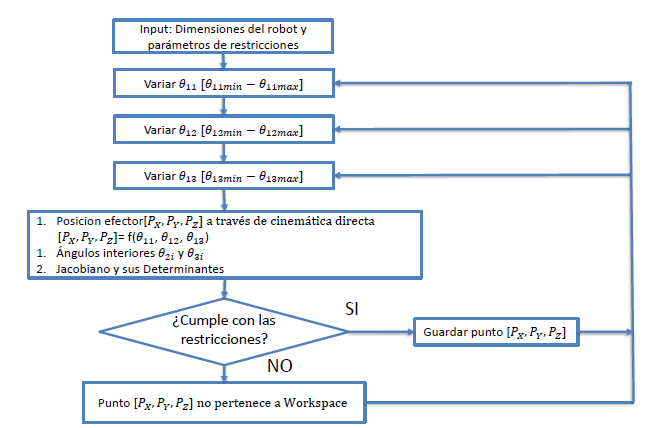
\includegraphics[width=1\linewidth]{Main/Chapter6/Images6/cap6_ws_2.png}
                \caption{Fotografía de un paraguas}
                \label{f:Cap6_ws_2}
            \end{figure}  

    CAMBIARDIAGRAMA La idea principal de la solución propuesta es calcular un grupo significativo de configuraciones $(P_x,P_y,P_z)$ posibles del efector final en base a sus dimensiones y evaluar si cumplen con restricciones impuestas. Se obtienen las configuraciones cartesianas del efector $(P_x,P_y,P_z)$  utilizando la cinemática directa y variando los angulos $\theta_{11}$,$\theta_{12}$,$\theta_{13}$ en los rangos $[\theta_{11min}-\theta_{11max}]$, $[\theta_{12min}-\theta_{12max}]$, $[\theta_{13min}-\theta_{13max}]$ respectivamente. Todos estos rangos se discretizan con un paso impuesto \(  \Delta  \theta _{1i} \). Si el punto  $(P_x,P_y,P_z)$ cumple con todas las restricciones, el punto pertenece al espacio de trabajo. Al contrario, si el punto no cumple con una o mas restricciones, este no pertenece al espacio de trabajo.

        \newpage

    Las restricciones son las mismas que las expuestas en la sección \ref{restriccionesWS}. El orden en que se verifican las restricciones se muestran en el siguiente diagrama de flujo:

             \begin{figure}[htb]
                \centering
                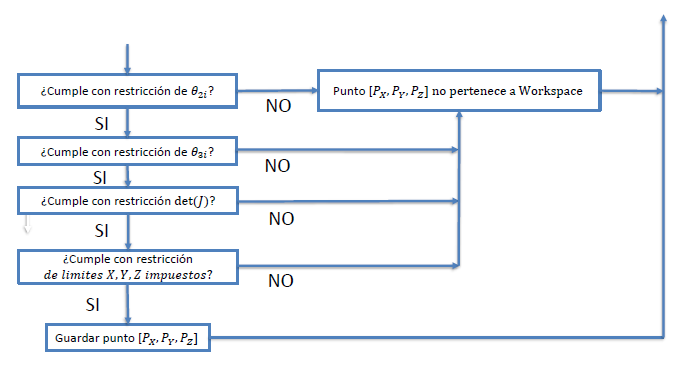
\includegraphics[width=1\linewidth]{Main/Chapter6/Images6/cap6_ws_3.png}
                \caption{Fotografía de un paraguas}
                \label{f:Cap6_ws_3}
            \end{figure}  


    Para calcular el espacio de trabajo se crea un nodo en ROS. La tarea especifica de este nodo es calcular, guardar y graficar los puntos $(P_x,P_y,P_z)$ del efector final que cumplen con las restricciones impuestas. 
    La representación gráfica del nodo se presenta en la ilustración \ref{f:Cap6_ws_1}: 
    
    
        % Define block styles
        \tikzstyle{block1} = [rectangle, draw=blue,fill=blue!20, text width=10em, text centered, minimum height=7em, minimum width=2.5em , text=black]
        \tikzstyle{block2} = [rectangle, draw=black!50,fill=black!20, text width=10em, text centered, minimum height=4em, minimum width=2.5em ]
        \tikzstyle{line} = [draw, -latex']
         \begin{center}
         \begin{figure}[htb]
             \begin{tikzpicture}[node distance = 5cm, auto]
                % Place nodes
                    \node [block1] (funcion) {\textbf{Espacio\\de\\Trabajo}};
                \node [block2, left of=funcion] (input) {\textbf{ $\Delta\theta _{1i}$\\$(Discretizacion$ $Espacio$ $Articular$$)$}};
                \node [block2, right of=funcion] (ouput) {\textbf{$\mathcal{W}_{(J_{x},J_{\theta})},\mathcal{W}_{J_{x}},\\\mathcal{W}_{J_{\theta}},\mathcal{W}_{(J_{x},J_{\theta},Limites)}$\\($Espacios$ $de$ $Trabajo$ $en$ $coordenadas$ $cartesianas$ $y$ $articular$)}};
                % Draw edges
                \path [line] (funcion) -- node {}(ouput);
                \path [line] (input) -- node { }(funcion);
            \end{tikzpicture}
                \caption{Fotografía de un paraguas}
                \label{f:Cap6_ws_1}
         \end{figure}
         \end{center}
         
        \vspace{-1cm}         
    
    En este nodo, las dimensiones del robot y las restricciones son establecidas antes de calcular el espacio de trabajo. La única entrada es el paso de la discretizacion de los rangos \(  \Delta  \theta _{1i} \). La cinematica directa y el jacobiano se calculan a partir del método A, específicamente los desarrollados en las secciones \ref{ma_cd} y \ref{ma_jac} respectivamente. Se emplea este método por la razón de que el jacobiano $J$ se puede bipartir en dos matrices $(J_{x}$  y  $J_{ \theta })$, donde cada una de ellas representa una singularidad especifica . Ademas, el metodo A tiene la ventaja que tiene las ecuaciones para determinar los ángulos interiores $\theta_{2i}$ y $\theta_{3i}$.
    
    \newpage
    
    El valor de los parámetros de las restricciones impuestas en este trabajo de grado se presentan y se explican en la tabla \ref{t:cap6_ws_1}: 
    
            \begingroup
            \renewcommand{\arraystretch}{1.5}
            \begin{table}[H]
            \centering
            \begin{tabular}{c m{7.5cm} c c}
               \hline
               \textbf{Restriccion}  & \textbf{Explicacion} & \textbf{Min}& \textbf{Max}\\
               \hline           \hline            
             $\theta_{1i}$ & Colisión entre los brazos y la base fija & $-90^{\circ}$ & $90^{\circ}$\\
            \hline
             $\Delta\theta _{1i}$ & Pasos de discretizacion de rangos $\theta_{1i}$ muy bajos implica costo computacional alto& $5^{\circ}$ & $ $ \\
            \hline
             $\theta _{2i}$ & Angulo debe ser menor a $180^{\circ}$ ya que en esa situación el brazo y antebrazo podrían ser colineales y producir singularidades. Ademas esta restriccion asegura que el calculo de la cinemática de posición sea la correcto ya que descarta una de las soluciones & $5^{\circ}$ & $175^{\circ}$ \\
            \hline
             $\theta _{3i}$ & Angulo respecto a la inclinación máxima de las rotulas por catalogo, generalmente son de $13^{\circ}$ & $45^{\circ}$ & $135^{\circ}$ \\
            \hline
             $J_{x}$ & Depende de la precisión o factor de seguridad subjetivo& $6*10^{-1}$ & $ $ \\
            \hline
             $J_{\theta}$ & Depende de la precisión o factor de seguridad subjetivo& $4*10^{-3}$ & $ $ \\
            \hline
             $X$ & Limite X de espacio de trabajo impuesto por el fabricante & $-400[mm]$ & $+400[mm]$ \\
            \hline            
             $Y$ & Limite Y de espacio de trabajo impuesto por el fabricante & $-400[mm]$ & $+400[mm]$ \\
            \hline   
             $Z$ & Limite Z de espacio de trabajo impuesto por el fabricante & $-300[mm]$ & $-750[mm]$ \\
            \hline   
            \end{tabular}
            \caption{Referencias del dibujo}
            \label{t:cap6_ws_1}
        \end{table}
        \endgroup     
        
         \begin{figure}[htb]
                \centering
                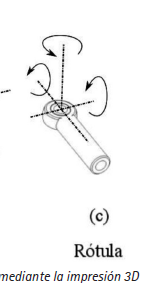
\includegraphics[width=0.1\linewidth]{Main/Chapter6/Images6/cap6_ws_4.png}
                \caption{Fotografía de un paraguas}
                \label{f:Cap6_ws_4}
            \end{figure}    
    
        \newpage

    El siguiente algoritmo presenta el pseudocódigo de la función dentro del nodo que determinar el espacio de trabajo:
    
\begin{algorithm}[H]
    \caption{Espacio de Trabajo} 
    \SetKwInput{KwInput}{Input}                % Set the Input
    \SetKwInput{KwOutput}{Output}              % set the Output
    \SetKwInput{KwObjetivo}{Objetivo}                % Set the Input
    \SetKwInput{Kwfile}{Nombre archivo}                % Set the Input
    
    \DontPrintSemicolon
      \KwObjetivo {Encontrar el espacio de trabajo del robot delta a partir de sus dimensiones y restricciones impuestas.}
      \Kwfile{$workspace\_v2.py$}
      \KwInput{ $\Delta\theta _{1i}$}
      \KwOutput{$[\mathcal{W}_{(J_{x},J_{\theta})},\mathcal{W}_{J_{x}},\mathcal{W}_{J_{\theta}},\mathcal{W}_{(J_{x},J_{\theta},Limites)}]$}
      
      % Set Function Names{\theta }_1,{\theta }_2,{\theta }_3
      \SetKwFunction{FSub}{espaciotrabajo}
       \SetKwProg{Fn}{}{:}{}
    
      \tcc{FUNCION PRINCIPAL}
        \Fn{\FSub{$\Delta\theta _{1i}$}}{
            \tcc{Barrido de angulos $\theta _{11}$ , $\theta _{12}$ y $\theta _{13}$ con incrementos de $\Delta\theta _{1i}$}
            \For{\theta _{11} \in [$\theta_{11min}$ - $\theta_{11max}]$;$\Delta\theta _{1i}$}    
                { 
                \For{\theta _{12} \in [$\theta_{12min}$ - $\theta_{12max}]$;$\Delta\theta _{1i}$}  
                    { 
                    \For{\theta _{13} \in [$\theta_{13min}$ - $\theta_{13max}]$;$\Delta\theta _{1i}$}    
                        { 
                        \tcc{Cinematica Directa}
                	     $(P_{x},P_{y},P_{z})=forward(\theta _{12},\theta _{13},\theta _{11})$\;
                        \tcc{Jacobiano}
                        $[J_{\theta},J_{x},\theta_{31},\theta_{32},\theta_{33},\theta_{21},\theta_{22},\theta_{23},J] = jacobian\_total(P_{x},P_{y},P_{z},\theta_{11},\theta_{12},\theta_{13})   $\;
                        \tcc{Determinantes Jacobiano}
                        $\left|J_{\theta}\right|=det(J_{\theta})$\;
                        $\left|J_{x}\right|=det(J_{x})$\;
                         \tcc{Restricciones}
                          \If {$Restricciones$ $\theta_{2i}$} 
                              {
                                \If {$Restricciones$ $\theta_{3i}$} 
                                      {
                                      \If {$Restricciones$ $\left|J_{x}\right|$ o $\left|J_{\theta}\right|$} 
                                              {
                                              $\mathcal{W}_{(J_{x},J_{\theta})} =(P_{x},P_{y},P_{z},\theta_{11},\theta_{12},\theta_{13})$ \;
                                                  \If {$Restricciones$ $Limites XYZ$} 
                                                  { $\mathcal{W}_{(J_{x},J_{\theta},limites)}=(P_{x},P_{y},P_{z},\theta_{11},\theta_{12},\theta_{13})$ \;
                                                  }
                                              }
                                        \Else{$(P_{x},P_{y},P_{z})$ No pertenece al espacio de trabajo\;}
                                      \If {$Restricciones$ $\left|J_{x}\right|$} 
                                              {
                                               $\mathcal{W}_{J_{x}}=(P_{x},P_{y},P_{z},\theta_{11},\theta_{12},\theta_{13})$
                                              }
                                      \If {$Restricciones$ $\left|J_{\theta}\right|$} 
                                              {
                                               $\mathcal{W}_{J_{\theta}} =(P_{x},P_{y},P_{z},\theta_{11},\theta_{12},\theta_{13})$
                                              }
                                      
                                    }
                              }
                        }  
                    }           
                }
                       \KwRet  $[\mathcal{W}_{(J_{x},J_{\theta})},\mathcal{W}_{J_{x}},\mathcal{W}_{J_{\theta}},\mathcal{W}_{(J_{x},J_{\theta},Limites)}]$\;
            }
\end{algorithm}
    
    \newpage

    \subsection{Trayectoria}
    
    En esta seccion se explica el desarrollo para determinar la trayectoria en el espacio articular del robot delta, es decir, la trayectoria angular de los actuadores, a partir de una trayectoria lineal interpolada en el espacio cartesiano XYZ que recorre el efector final de un punto inicial $P_i$ a un punto final $P_f$ con restricciones de velocidad trapezoidal en dirección del camino geometrico.

        % Define block styles
        \tikzstyle{block1} = [rectangle, draw=blue,fill=blue!20, text width=10em, text centered, minimum height=5em, minimum width=2.5em , text=black]
        \tikzstyle{block2} = [rectangle, draw=black!50,fill=black!20, text width=10em, text centered, minimum height=4em, minimum width=2.5em ]
        \tikzstyle{line} = [draw, -latex']
         \begin{center}
         \begin{figure}[htb]
             \begin{tikzpicture}[node distance = 5cm, auto]
                % Place nodes
                    \node [block1] (funcion) {\textbf{Trayectoria}};
                \node [block2, left of=funcion] (input) {\textbf{$P_i$ $P_f$}};
                \node [block2, right of=funcion] (ouput) {\textbf{$Puntos$ $de$ $la$ \\ $Trayectoria$ \\$en$ $el$\\ $espacio$\\ $cartesiano$ $XYZ$}};
                % Draw edges
                \path [line] (funcion) -- node {}(ouput);
                \path [line] (input) -- node { }(funcion);
            \end{tikzpicture}
                \caption{Fotografía de un paraguas}
                \label{f:cap6_trayectory_1}
         \end{figure}
         \end{center}
         
        \vspace{-1cm}   

        
    Esta trayectoria se compone de un camino geométrico lineal en el espacio cartesiano XYZ se llaman 'punto a punto en linea recta' y la escala temporal es de 'Perfil de Movimiento Trapezoidal respecto a la Velocidad' o 'Linear segment with Parabolic Blends (LSPB)', visto en la sección \ref{cap4_tray}. 
    
    El perfil de movimiento trapezoidal visto en la sección \ref{Perfiles_de_movimiento_trapezoidal} se puede modificar para que las ecuaciones consideren el punto inicial y final especificando la velocidad máxima y la aceleracion maxima de la siguiente manera:
        \begin{equation}
        \Large
            q(t) = \left\lbrace
                \begin{array}{ll}
                q_0 + s\frac{a}{2}t^2&   0< t \leq \tau\\
                q_0 - s\frac{V^2}{2a}+sVt &  \tau< t \leq T- \tau\\
                q_1 + s \left( -\frac{aT^2}{2}+aTt-\frac{a}{2}t^2 \right) &  T- \tau< t \leq T\\
            \end{array}
            \right.
            \label{eq:cap6_tray_1}
        \end{equation}
    
    Donde:
    \begin{equation*}
       \text{$q_0$: $Punto$ $inicial$}
    \end{equation*}
    \begin{equation*}
       \text{$q_1$: $Punto$ $final$ }
    \end{equation*}
    \begin{equation*}
       \text{$V$: $velocidad$ $maxima$ $permitida$}
    \end{equation*}
    \begin{equation*}
       \text{$a$: $aceleracion$ $maxima$ $permitida$}
    \end{equation*}
    
    \newpage
    
    \begin{equation}
        \tau=\frac{V}{a}
    \label{eq:cap6_tray_4}
    \end{equation}
    \begin{equation}
        T=s\frac{q_1-q_0}{V}+\frac{V}{a}
    \label{eq:cap6_tray_5}
    \end{equation}
    \begin{equation}
        s=signo(q_1-q_0)
    \label{eq:cap6_tray_6}
    \end{equation}
    

     \begin{figure}[htb]
            \centering
            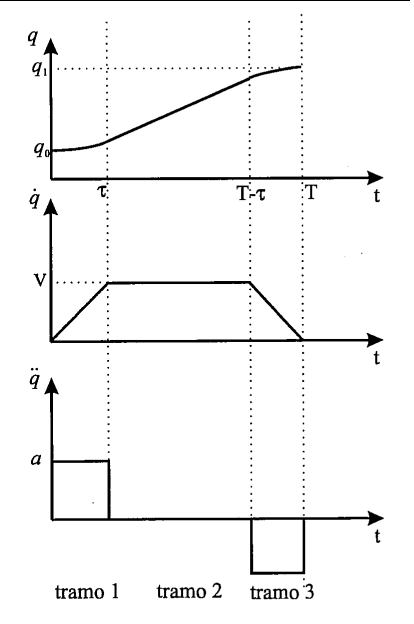
\includegraphics[width=0.7\linewidth]{Main/Chapter6/Images6/cap6_trayectory_2.png}
            \caption{Fotografía de un paraguas}
            \label{f:cap6_trayectory_2}
        \end{figure} 


    \newpage

    Para utilizar el perfil de velocidad trapezoidal en el camino geométrico lineal interpolado desde el punto inicial $P_i$ al punto final $P_f$ se aplican matrices de rotaciones. 
    
    
    \begin{enumerate}[1.]
        \item     Primero se traslada el sistema de referencia general $X_0Y_0Z_0$ al punto inicial $P_i$ generando un nuevo sistema de referencia $X_{trans}Y_{trans}Z_{trans}$ . 
        
        \item Luego se rota $X_{trans}Y_{trans}Z_{trans}$ sobre el eje $Z_{trans}$ en un angulo de $\theta_z$ generando un nuevo sistema de referencia $X_{rot_{\theta_z}}Y_{rot_{\theta_z}}Z_{rot_{\theta_z}}$. $\theta_z$  es el angulo interno entre el eje $X_{trans}$ y el vector   $\overrightarrow{$O_{X_{trans}Y_{trans}Z_{trans}}{P'}_f$}$ donde ${P'}_f$ es la  proyeccion de $P_f$ sobre el plano  $Y_{trans}Z_{trans}$.
        
        \item     Finalmente el marco de referencia $X_{rot_{\theta_z}}Y_{rot_{\theta_z}}Z_{rot_{\theta_z}}$ se rota sobre el eje  $Y_{rot_{\theta_z}}$ en un angulo de $\theta_y$ generando el ultimo sistema de referencia $X_{rot_{\theta_y}}Y_{rot_{\theta_y}}Z_{rot_{\theta_y}}$.
        $\theta_y$  es el angulo interno entre el eje $X_{rot_{\theta_z}}$ y el vector   $\overrightarrow{$O_{X_{rot_{\theta_z}}Y_{rot_{\theta_z}}Z_{rot_{\theta_z}}}{P''}_f$}$ donde ${P''}_f$ es el punto  ${P}_f$ con respecto al sistema de referencia  $X_{rot_{\theta_z}}Y_{rot_{\theta_z}}Z_{rot_{\theta_z}}$ .
         En el marco de referencia $X_{rot_{\theta_y}}Y_{rot_{\theta_y}}Z_{rot_{\theta_y}}$ se aplica el perfil de velocidad trapezoidal para que define la escala temporal de la trayectoria y la interpolación lineal en el espacio cartesiano del camino geométrico. 
    \end{enumerate}
    
     \begin{figure}[htb]
            \centering
            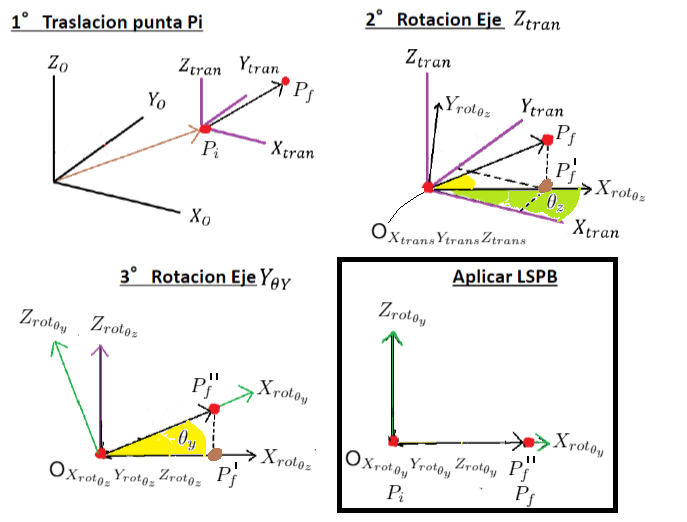
\includegraphics[width=1\linewidth]{Main/Chapter6/Images6/cap6_trayectory_3.png}
            \caption{Fotografía de un paraguas}
            \label{f:cap6_trayectory_3}
        \end{figure} 
        
    \newpage
        
    El diagrama de flujo para el desarrollo de la trayectoria se presenta en la ilustración \ref{f:cap6_trayectory_4}:
    
     \begin{figure}[htb]
            \centering
            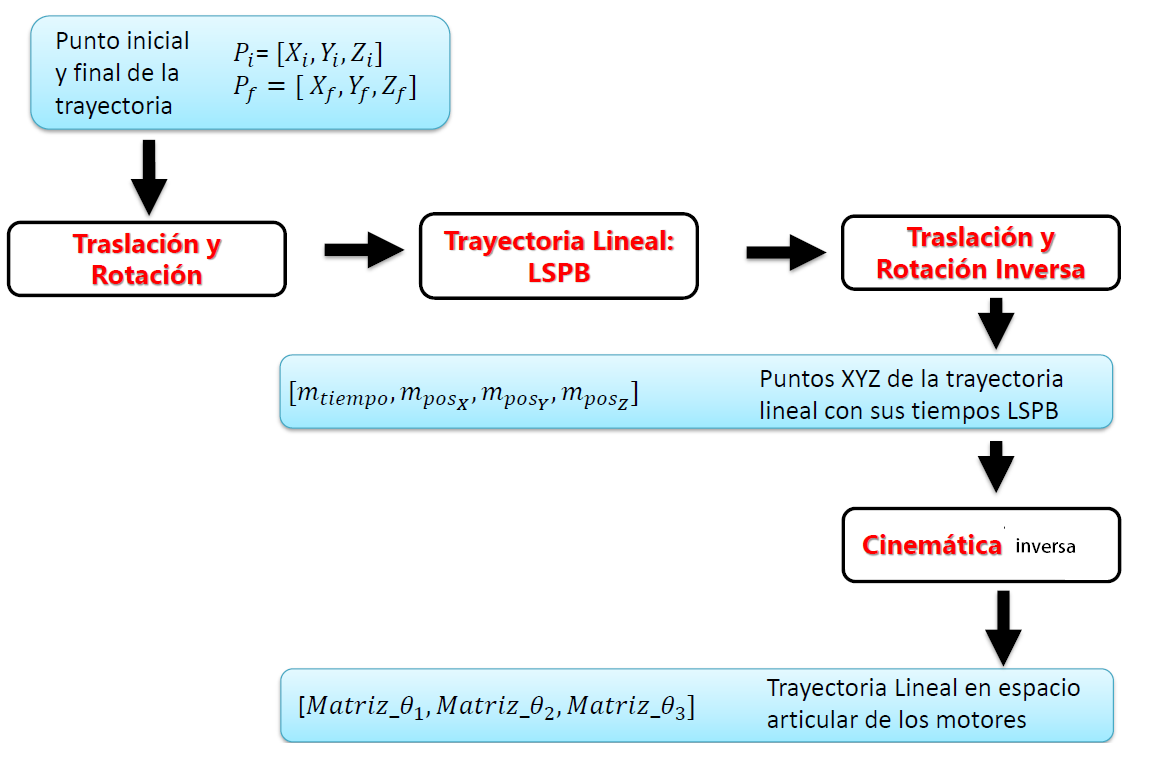
\includegraphics[width=1\linewidth]{Main/Chapter6/Images6/cap6_trayectory_4.png}
            \caption{Fotografía de un paraguas}
            \label{f:cap6_trayectory_4}
        \end{figure}
        
    A partir de de el punto inicial $P_i$ y el punto final $P_f$ se realiza una traslación y 2 rotaciones para aplicar la escala temporal de perfil trapezoidal y la interpolación del camino geométrico lineal. Luego se aplica traslación y rotaciones inversas para obtener la trayectoria en el espacio cartesiano respecto al sistema de referencia general.Finalmente se emplea la cinemática inversa para conseguir las trayectorias en el espacio articular de los actuadores.     
    
         \begin{figure}[htb]
            \centering
            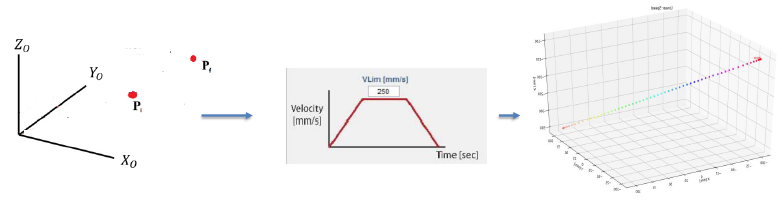
\includegraphics[width=0.9\linewidth]{Main/Chapter6/Images6/cap6_trayectory_1.png}
            \caption{Fotografía de un paraguas}
            \label{f:cap6_trayectory_5}
        \end{figure}    
    \newpage
    
    

    \begin{algorithm}[H]
            \caption{Trayectoria} 
            \SetKwInput{KwInput}{Input}                % Set the Input
            \SetKwInput{KwOutput}{Output}              % set the Output
            \SetKwInput{KwObjetivo}{Objetivo}                % Set the Input
            \SetKwInput{Kwfile}{Nombre archivo}                % Set the Input
            
            \DontPrintSemicolon
              \KwObjetivo {Escala de tiempo perfil de velocidad Trapezoidal LSPB e interpolación de camino geometrico lineal }
              \Kwfile{$linear\_speed\_f\_adams.py$}
              \KwInput{$q_0,q_1,v_{max},a_{max},{n}_{\Delta Tramo1},{n}_{\Delta Tramo2}$}
              \KwOutput{$tiempo,{X}_{rot_{\theta_y}},{\dot{X}}_{rot_{\theta_y}},{\ddot{X}}_{rot_{\theta_y}}$}
              
                % Set Function Names
              \SetKwFunction{FSum}{$ls\_v\_a\_total$}
              \SetKwFunction{FSub}{$ls\_v\_a\_puntual$}
            
              \tcc{FUNCION PRINCIPAL}
              \SetKwProg{Fn}{}{:}{}
              \Fn{\FSum{$q_0,q_1,v_{max},a_{max},{n}_{\Delta Tramo1},{n}_{\Delta Tramo2}$}}{
              \tcc{Parametros de Curva LSPB}
                ${n}_{\Delta Tramo3}={n}_{\Delta Tramo1}$  \tcp*{División Tramo 3 = Tramo 1}
            	$\tau=v_{max}/a_{max}$ \tcp*{Tiempo total del tramo 1 y tramo 3}
            	$s=signo(q1-q0)$\;
            	$T=s\frac{(q_1-q_0)}{v_{max}}+\tau$ \tcp*{Tiempo total de la trayectoria}
            	$\Delta_{tramo1}=(\tau)/{n}_{\Delta Tramo1}$\;
            	$\Delta_{tramo2}=(T-2\tau)/{n}_{\Delta Tramo2}$\;
            	$\Delta_{tramo3}=\Delta_{tramo1}$\;
            	$n_{total}=\sum_{i=1}^{3} n_{\Delta Tramoi}+1$\tcp*{Total puntos de discretizacion}

                \tcc{Verificar si alcanza la ${v}_{max}$ para {v}_{max}  }
            	$T_f=2\sqrt{\frac{q_1-q_0}{a_{max}}}$ \tcp*{Tiempo total de la trayectoria para ${a}_{max}$}
            	${v}_{max.por.acel}={a}_{max}(T_f/2)$\;
            	
                \If{{v}_{max.por.acel}\leq{v}_{max}}{
                		${v}_{max}={v}_{max.por.acel}$\;
                		$\tau=T_f/2$\;
                		$T=T_f$\;
                		$\Delta_{tramo1}=(\tau)/n_{\Delta Tramo1}$\;
                		$\Delta_{tramo2}=0$\;
                		${n}_{\Delta Tramo2}=0$\;
                		$n_{total}=\sum_{i=1}^{3} n_{\Delta Tramoi}+1$\;
                       }
                \tcc{Calulcar Curva LSBP}
                \For{ $i$ $in$ $range[0, n_{total}]$}    
                { 
                    $tiempo_i=tiempo_i+\Delta_{tramoi}$ \tcp*{$\Delta_{tramoi}$ depende de $i$}
            		$X=ls\_v\_a\_puntual(q_0,q_1,v_{max},a_{max},tiempo_i)$ \tcp*{LSPB}
            		\tcc{Resultados Posición,Velocidad,Aceleración de LSBP}
            		$ ({X}_{rot_{\theta_y}}[i],{\dot{X}}_{rot_{\theta_y}}[i],{\ddot{X}}_{rot_{\theta_y}}[i])=(X[0],X[1],X[2])$\;
            		$tiempo[i]=tiempo_i$\;
                }
               \KwRet $[tiempo,{X}_{rot_{\theta_y}},{\dot{X}}_{rot_{\theta_y}},{\ddot{X}}_{rot_{\theta_y}}]$
              }
    \end{algorithm}
    
    \clearpage   
        
\begin{algorithm}
      \ContinuedFloat
      \caption{Trayectoria (Continuacion...)}
      \tcc{SUBFUNCIONES}
      \SetKwProg{Fn}{}{:}{}
      \Fn{\FSub{$q_0,q_1,v_{max},a_{max},{tiempo}_{actual}$}}{
            	$\tau=v_{max}/a_{max}$\;
            	$s=signo(q_1-q_0)$\;
            	$T=s\frac{(q_1-q_0)}{v_{max}}+\tau$\;
        \tcc{Ecuaciones  LSPB (\ref{eq:cap6_tray_1})}
        \tcc{Tramo 1}
          \If{$(0 \leq {tiempo}_{actual}\leq \tau)$}
            {
        		$q_{actual}=q_0+s\frac{a_{max}}{2}{({tiempo}_{actual})}^2$\;
        		$v_{actual}=s{a}_{max}({tiempo}_{actual})$\;
        		$a_{actual}=s{a}_{max}$\;
        		$ \KwRet[q_{actual},v_{actual},a_{actual}]$\;
            }
        \tcc{Tramo 2}
            \ElseIf{$(\tau < {tiempo}_{actual}\leq T-\tau)$}
            {
        		$q_{actual}=q_0-(s\frac{{v_{max}}^2}{2{a}_{max}})+(s*{v}_{max}*{tiempo}_{actual})$\;
        		$v_{actual}=s*{v}_{max}$\;
        		$a_{actual}=0$\;
        		$ \KwRet[q_{actual},v_{actual},a_{actual}]$\;
            }
        \tcc{Tramo 3}
            \ElseIf{$(T-\tau<{tiempo}_{actual}\leq T)$}
            {
        		$q_{actual}=q_1+s\left(-\frac{a_{max}T^2}{2}+a_{max}T({tiempo}_{actual})-\frac{a_{max}}{2}{({tiempo}_{actual})}^2\right)$\;
        		$v_{actual}=s(a_{max}T-a_{max}{tiempo}_{actual})$\;
        		$a_{actual}=s(-a_{max})$\;
        		$\KwRet[q_{actual},v_{actual},a_{actual}]$\;
            }
      }
\end{algorithm}
    
        \newpage
    
    

    \newpage

\section{Interfaz de visualización Rviz}

    Rviz da la posibilidad de visualizar los componentes mecánicos de un robot de una forma mas simple. En esta tesis se desea simular una trayectoria lineal de la plataforma móvil de un robot delta. Para cumplir con dicho objetivo se necesitan en cada momento de la trayectoria los ángulos de las juntas que unen los componentes y la posición xyz del centroide de la plataforma móvil. La posición en el espacio de los brazos y antebrazos se determinan a partir de los ángulos de cada junta relativos a otras partes mecánicas y la posición de la plataforma móvil se determina mediante las coordenadas de su centroide xyz relativo al sistema de referencia global. Por lo tanto, como se configura la visualización de las partes mecánicas en 2 grupos por separado, si la cinemática inversa es correcta, entonces la plataforma móvil debe calzar perfectamente entre las rotulas (final de los antebrazos) que unen los antebrazos con la plataforma móvil.
     
   \subsection{Conexion ROS - RVIZ}
   
           Básicamente se puede obtener la visualización de la trayectoria del robot delta en 3 pasos:


            % Define block styles
        \tikzstyle{block1} = [rectangle, draw=black!50,fill=blue!20, text width=11em, text centered, minimum height=4em, minimum width=2.5em ]
        \tikzstyle{block2} = [rectangle, draw=black!50,fill=red!20, text width=11em, text centered, minimum height=4em, minimum width=2.5em ]
        \tikzstyle{block3} = [rectangle, draw=black!50,fill=yellow!20, text width=10em, text centered, minimum height=4em, minimum width=2.5em ]
        
        \tikzstyle{line} = [draw, -latex']
         \begin{center}
         \begin{figure}[htb]
             \begin{tikzpicture}[node distance = 5cm, auto]
                % Place nodes
                    \node [block1] (funcion) {\textbf{TF \\ $Nombre$  $Juntas$  $URDF$}};
                \node [block2, left of=funcion] (input) {\textbf{Trayectoria ROS \\ $\theta_{i=1,2,3}$\\$XYZ$\\ $   s(t)$\\ $\theta_{2i}$ \\ $\theta_{3i}$\\$Nombre$  $Juntas$  $URDF$ }};
                \node [block3, right of=funcion] (ouput) {\textbf{URDF y Rviz}};
                % Draw edges
                \path [line] (funcion) -- node {}(ouput);
                \path [line] (input) -- node { }(funcion);
            \end{tikzpicture}
                \caption{Fotografía de un paraguas}
                \label{f:cap6_trayectory_1}
         \end{figure}
         \end{center}
         
        \vspace{-1cm}   
        
        \begin{itemize}
            \item {Paso 1: Exportar de la trayectoria creada en ROS los siguientes datos: las posiciones de los motores $\theta_{i=1,2,3}$ , la posiciones del centroide de la plataforma móvil $XYZ$ y la escala de tiempo utilizada $s(t)$. Luego se determinan los ángulos interiores $\theta_{2i}$ y $\theta_{3i}$ (vistos en la sección \ref{cap4_angulosinteriores}) de las 3 cadenas cinemáticas. Esto es posible creando un nodo llamado $posicionador\_rviz\_realtime\_tm1\_adams$ que espera como datos de entrada los datos de la trayectoria  $\theta_{i=1,2,3}$, $XYZ$ y $s(t)$ y como salida da como resultado un objeto de tipo $JointState()$. Este ultimo objeto contiene los datos de los ángulos interiores en radianes, ángulo de los motores en radianes y la posición xyz de la plataforma móvil en metros. Además, cada ángulo y coordenada se le asigna un nombre único de tipo string, los cuales son usados para relacionar las juntas configuradas para el visualizador con respecto al valor de cada una de ellas a través de la trayectoria.}
            \item {Paso 2: Pasar a valores TF cada junta y coordenada adquirida del paso 1. Rviz tiene un nodo integrado llamada $estados\_robot\_pub.py$ que tiene como requisito de entrada los valores de cada junta con cada nombre único respectivamente y como salida da como resultado los valores TF con cada nombre unico respectivamente}
            \item {Paso 3: Anterior a crear una trayectoria en ROS se debe configurar el robot delta en formato URDF. Los nombres de cada juntas en el archivo urdf en formato xml deben ser exactamente los mismo que en los pasos 1 y 2}
        \end{itemize}
        

            Los nombres de cada junta se muestran en la siguiente tabla: 
            
        \begingroup
            \renewcommand{\arraystretch}{1.5}
            \begin{table}[H]
                \centering
                \begin{tabular}{|c|m{2.5cm}|m{8cm}|}
                   \hline
                   \textbf{Simbología}  &  \textbf{Nombre}  & \textbf{Descipcion}    \\\hline
                   $\theta_{11}$  & base\_brazo1    & Ángulo del motor en cadena cinemática 1                       \\\hline
                   $\theta_{12}$  & base\_brazo2    & Ángulo del motor en cadena cinemática 2                            \\\hline
                   $\theta_{13}$  & base\_brazo3    & Ángulo del motor en cadena cinemática 3                            \\\hline
                   $\theta_{21}$  & codo1\_a    & Ángulo interior 2 de la rotula que une el brazo con el antebrazo en cadena cinemática 1                       \\\hline
                   $\theta_{31}$  & codo1\_b    & Ángulo interior 3 de la rotula que une el brazo con el antebrazo en cadena cinemática 1                       \\\hline
                   $\theta_{22}$  & codo2\_a    & Ángulo interior 2 de la rotula que une el brazo con el antebrazo en cadena cinemática 2                       \\\hline
                   $\theta_{32}$  & codo2\_b    & Ángulo interior 3 de la rotula que une el brazo con el antebrazo en cadena cinemática 2                       \\\hline
                   $\theta_{23}$  & codo3\_a    & Ángulo interior 2 de la rotula que une el brazo con el antebrazo en cadena cinemática 3                       \\\hline
                   $\theta_{33}$  & codo3\_b    & Ángulo interior 2 de la rotula que une el brazo con el antebrazo en cadena cinemática 3                       \\\hline
                   $X$  & act\_x    & Posición X del centroide de la plataforma móvil                       \\\hline
                   $Y$  & act\_y    & Posición Y del centroide de la plataforma móvi                       \\\hline
                   $Z$  & act\_z    & Posición Z del centroide de la plataforma móvi                       \\\hline

                \end{tabular}
                \caption{Referencias del dibujo}
                \label{tab:cap6_rviz_1}
            \end{table}
        \endgroup

    \newpage
       
       
       
    \subsection{Modelo URDF}
        Para visualizar un modelo de un robot se usa un archivos de formato de descripción de robot unificado (URDF) basados en XML. En esta sección se presenta la configuración del modelo del robot delta mostrando el código para los enlaces, juntas y la respectiva unión padre-hijo para cada uno de ellos. La nomenclatura utilizada es la del capitulo \ref{CAP5}. El nombre del archivo donde estan contenidos todos estos codigos es robot.urdfm1.adams.urdf.  
        
       \subsubsection{Base Fija}
        La base fija es un enlace que se le nombra \textbf{"base\_link"} y se representa como un cilindro de radio \textbf{$R_a$}.

             \begin{figure}[h]
                \centering
                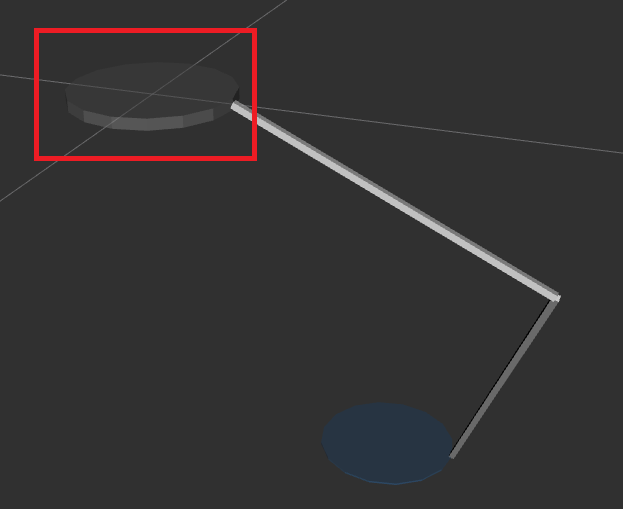
\includegraphics[width=0.6\linewidth]{Main/Chapter6/Images6/cap6_basefija.png}
                \caption{Fotografía de un paraguas}
                \label{f:Cap6_urdf_1}
            \end{figure}  


        \lstset{language=XML}
        \begin{lstlisting}
<!--BASE SUPERIOR:____________________-->
<link name="base_link">
	<visual>
		<geometry>
			<cylinder length="0.005" radius="0.210"/> 
		</geometry>
		<material name="gris">
			<color rgba="0.55 0.55 0.55 0.5"/>
		</material>
	</visual>
</link>
        \end{lstlisting}

      \newpage

       \subsubsection{Brazos}
        Los brazos son enlaces que se le nombra \textbf{"brazo1 , brazo2 y brazo3"} y se representan como un paralelepípedo tipo box de largo \textbf{$L_a$}. Estos brazos se unen a la base fija a través de una junta tipo revoluta que representan los motores o actuadores del robot delta. Las juntas se les asignan los nombres \textbf{"base\_brazo1 , base\_brazo2 y base\_brazo3"} para cada brazo respectivamente. En el código de las juntas se configura las conexiones padre-hijo.
        
        
             \begin{figure}[h]
                \centering
                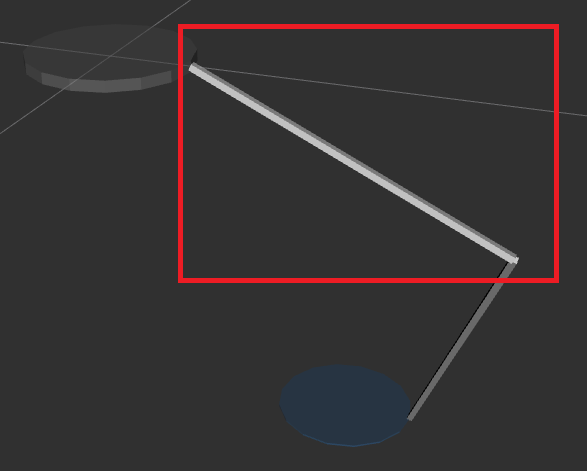
\includegraphics[width=0.4\linewidth]{Main/Chapter6/Images6/cap6_brazo.png}
                \caption{Fotografía de un paraguas}
                \label{f:Cap6_urdf_2}
            \end{figure}  
            

        \lstset{language=XML}
        \begin{lstlisting}
<!--BRAZOS SUPERIORES:____________________-->
<!--BRAZO_1-->
<link name="brazo1">
	<visual>
		<origin xyz="0.310 0 0" rpy="0 0 0"/> <!--La/2-->
		<geometry>
			<box size="0.620 0.003 0.003"/> <!--La -->
		</geometry>
		<material name="blanco">
			<color rgba="0.9 0.9 0.9 1"/>
		</material>
	</visual>
</link>
<joint name="base_brazo1" type="revolute">
	<axis xyz="0 1 0"/>
	<limit effort="100.0" lower="0.0" upper="1.8" velocity="0.5"/>
	<parent link="base_link"/>
	<child link="brazo1"/>
	<origin xyz="-0.181865335 0.105 0" rpy="0 0 2.61799"/> 
</joint>

<!--BRAZO_2-->
<link name="brazo2">
	<visual>
		<origin xyz="0.310 0 0" rpy="0 0 0"/> <!--La/2-->
		<geometry>
			<box size="0.620 0.003 0.003"/>  <!--La -->
		</geometry>
		<material name="blanco"/>
	</visual>
</link>

<joint name="base_brazo2" type="revolute">
	<axis xyz="0 1 0"/>
	<limit effort="100.0" lower="0.0" upper="1.8" velocity="0.5"/>
	<parent link="base_link"/>
	<child link="brazo2"/>
	<origin xyz="0 -0.210 0" rpy="0 0 -1.57075"/> 
</joint>

<!--BRAZO_3-->
<link name="brazo3">
	<visual>
		<origin xyz="0.310 0 0" rpy="0 0 0"/><!--La/2-->
		<geometry>
			<box size="0.620 0.003 0.003"/> <!--La -->
		</geometry>
		<material name="blanco"/>
	</visual>
</link>
<joint name="base_brazo3" type="revolute">
	<axis xyz="0 1 0"/>
	<limit effort="100.0" lower="0.0" upper="1.8" velocity="0.5"/>
	<parent link="base_link"/>
	<child link="brazo3"/>
	<origin xyz="0.181865335 0.105 0" rpy="0 0 0.523599"/> 
</joint>
        \end{lstlisting}
        
        \newpage

       
       \subsubsection{Antebrazos}
       
        Los antebrazos son enlaces que se le nombra \textbf{"barra1\_b , barra2\_b y barra3\_b"} y se representan como un paralelepípedo tipo box de largo \textbf{$L_b$}. Estos antebrazos se unen cada uno a su respectivo brazo través de 2 junta tipo revoluta que representan rotulas. Las juntas se les asignan los nombres \textbf{' codo1\_a , codo1\_b , codo2\_a , codo2\_b , codo3\_a , codo3\_b'} para cada brazo respectivamente. En el código de las juntas se configura las conexiones padre-hijo que determina al fin y al cabo la posición de los antebrazos respecto al brazo.
        
        \begin{figure}[h]
                \centering
                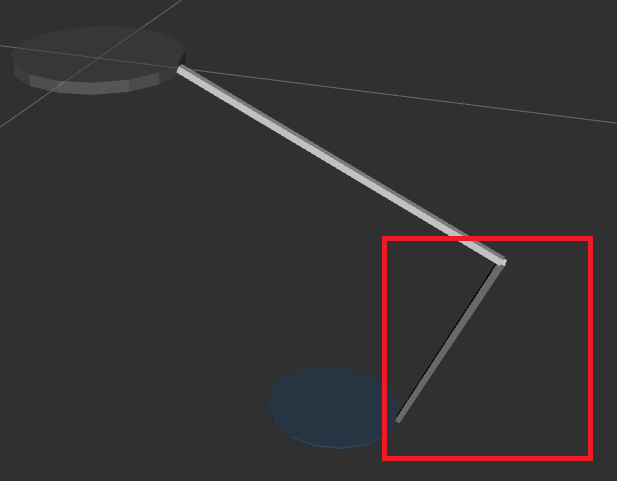
\includegraphics[width=0.4\linewidth]{Main/Chapter6/Images6/cap6_antebrazo.png}
                \caption{Fotografía de un paraguas}
                \label{f:Cap6_urdf_3}
            \end{figure}
        
        \lstset{language=XML}
        \begin{lstlisting}
<!--BRAZOS INFERIORES:____________________-->	
<!--Ante_BRAZO_1-->
<link name="barra1_a"/>
<joint name="codo1_a" type="revolute">
	<axis xyz="0 -1 0"/>
	<limit effort="100.0" lower="-3.14" upper="3.14" velocity="0.5"/>
	<parent link="brazo1"/>
	<child link="barra1_a"/>
	<origin xyz="0.620 0 0" rpy="0 0 0"/>
</joint>
<link name="barra1_b">
	<visual>
		<origin xyz="-0.440 0 0" rpy="0 0 0"/> <!--Lb/2-->
		<geometry>
			<box size="0.880 0.003 0.003"/> <!--Lb-->
		</geometry>
		<material name="blanco"/>
	</visual>
</link>
<jonti name="codo1_b" type="revolute">
	<axis xyz="0 0 1"/>
	<limit effort="100.0" lower="-3.14" upper="3.14" velocity="0.5"/>
	<parent link="barra1_a"/>
	<child link="barra1_b"/>
	<origin xyz="0 0 0" rpy="0 0 0"/> 
</joint>

<!--Ante_BRAZO_2-->
<link name="barra2_a"/>
<joint name="codo2_a" type="revolute">
	<axis xyz="0 -1 0"/>
	<limit effort="100.0" lower="-3.14" upper="3.14" velocity="0.5"/>
	<parent link="brazo2"/>
	<child link="barra2_a"/>
	<origin xyz="0.620 0 0" rpy="0 0 0"/> <!--la = 150-->
</joint>
<link name="barra2_b">
	<visual>
		<origin xyz="-0.440 0 0" rpy="0 0 0"/> <!--Lb-/2->
		<geometry>
			<box size="0.880 0.003 0.003"/> <!--Lb-->
		</geometry>
		<material name="blanco"/>
	</visual>
</link>
<joint name="codo2_b" type="revolute">
	<axis xyz="0 0 1"/>
	<limit effort="100.0" lower="-3.14" upper="3.14" velocity="0.5"/>
	<parent link="barra2_a"/>
	<child link="barra2_b"/>
	<origin xyz="0 0 0" rpy="0 0 0"/> <!--O2 = 62.0652 -107.5000 0-->
</joint>

<!--Ante_BRAZO_3-->
<link name="barra3_a"/>
<joint name="codo3_a" type="revolute">
	<axis xyz="0 -1 0"/>
	<limit effort="100.0" lower="-3.14" upper="3.14" velocity="0.5"/>
	<parent link="brazo3"/>
	<child link="barra3_a"/>
	<origin xyz="0.620 0 0" rpy="0 0 0"/> <!--O2 = 62.0652 -107.5000 0-->
</joint>
<link name="barra3_b">
	<visual>
		<origin xyz="-0.440 0 0" rpy="0 0 0"/><!--Lb-/2->
		<geometry>
			<box size="0.880 0.003 0.003"/> <!--Lb-->
		</geometry>
		<material name="blanco"/>
	</visual>
</link>
<joint name="codo3_b" type="revolute">
	<axis xyz="0 0 1"/>
	<limit effort="100.0" lower="-3.14" upper="3.14" velocity="0.5"/>
	<parent link="barra3_a"/>
	<child link="barra3_b"/>
	<origin xyz="0 0 0" rpy="0 0 0"/> <!--O2 = 62.0652 -107.5000 0-->
</joint>

        \end{lstlisting}
       
%               \newpage

       \subsubsection{Base Movil}

        La base movil es un enlace que se le nombra \textbf{'actuador'} y se representa como un cilindro de radio \textbf{$R_b$}. La posición y orientación de este enlace no es respecto a ningún otro enlace, solo se determina en relación al sistema de referencia global. Para posicionar el centroide del cilindro, se utilizan 3 juntas tipo prisma, que representan las coordenadas x,y,z. Los nombres de estas juntas son \textbf{'act\_x','act\_y' y 'act\_z'}-

        \begin{figure}[h]
                \centering
                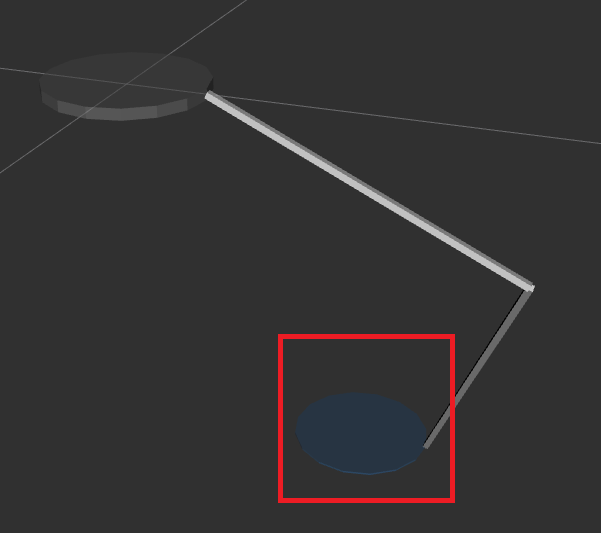
\includegraphics[width=0.4\linewidth]{Main/Chapter6/Images6/cap6_basemovil.png}
                \caption{Fotografía de un paraguas}
                \label{f:Cap6_urdf_4}
            \end{figure}

        \lstset{language=XML}
        \begin{lstlisting}
<link name="actuador">
	<visual>
		<origin xyz="0 0 0" rpy="0 -1.57075 0"/>
		<geometry>
			<cylinder length="0.001" radius="0.050"/>
		</geometry>
		<material name="colorte">
			<color rgba="0.15 0.55 0.95 0.3"/>
		</material>
	</visual>
</link>
<link name="aux1"/>
<link name="aux2"/>
<joint name="act_x" type="prismatic">
	<parent link="base_link"/>
	<child link="aux1"/>
	<limit effort="100.0" lower="-1" upper="1" velocity="0.5"/>
	<origin rpy="0 0 0" xyz="0 0 0"/>
</joint>
<joint name="act_y" type="prismatic">
	<parent link="aux1"/>
	<child link="aux2"/>
	<limit effort="100.0" lower="-1" upper="1" velocity="0.5"/>
	<origin rpy="0 0 1.57075" xyz="0 0 0"/>
</joint>
<joint name="act_z" type="prismatic">
	<parent link="aux2"/>
	<child link="actuador"/>
	<limit effort="100.0" lower="0" upper="1" velocity="0.5"/>
	<origin rpy="0 -1.57075 0" xyz="0 0 0"/>
</joint>
        \end{lstlisting}

      \newpage
  
  



    \newpage


\section{ADAMS}
